% ----------------------------------------------------------------------------------------------------------
% Praeambel
% ----------------------------------------------------------------------------------------------------------
\documentclass[fontsize=12pt,%
paper=a4,%
DIV=classic,%
%BCOR=10mm,%
twoside=true,%
headings=openany,%
parskip=half+,%
pagesize=auto,%
numbers=noenddot,%
headsepline=true,%
toc=listof,%
toc=bibliography%
]{scrreprt}

% PDF-Kompression
\pdfminorversion=5
\pdfobjcompresslevel=1

% Schriften
%\usepackage{mathpazo,tgpagella}
%\usepackage{libertine}
%\usepackage{fourier}
\usepackage{lmodern}

% Allgemeines
\usepackage{amsmath,amssymb} % Mathesachen
\usepackage[T1]{fontenc} % Ligaturen, richtige Umlaute im PDF
\usepackage[utf8]{inputenc}% UTF8-Kodierung für Umlaute usw

\usepackage{siunitx}
\usepackage{scrlayer-scrpage} 
\pagestyle{scrheadings}

%\usepackage{setspace}
%\onehalfspacing 

% Schriften-Größen
\setkomafont{chapter}{\Huge\rmfamily}
\setkomafont{section}{\Large\rmfamily}
\setkomafont{subsection}{\large\rmfamily}
\setkomafont{subsubsection}{\large\rmfamily}
\setkomafont{chapterentry}{\large\rmfamily} % Überschrift der Ebene in Inhaltsverzeichnis
\setkomafont{descriptionlabel}{\bfseries\rmfamily} % für description Umgebungen
\setkomafont{captionlabel}{\small\bfseries}
\setkomafont{caption}{\small}

% Sprache: Deutsch
\usepackage[autostyle,babel,german=guillemets,style=german]{csquotes}
\usepackage[USenglish,ngerman]{babel} 
\selectlanguage{ngerman}
% PDF
\usepackage[ngerman,%
pdfauthor={B. Ternes, J. Feldkamp},%
pdftitle={Modellbasierte Implementierung einer Vektorregelung für Synchronmaschinen},%
colorlinks=true,linkcolor=blue,citecolor=blue,filecolor=magenta,urlcolor=blue%
]{hyperref}

% BibLaTeX
\usepackage[backend=biber,%
 style=authoryear,%
 bibstyle=authoryear,%
 citestyle=authoryear,%
 % autocite=inline,%
 sorting=anyt,%
 sortcites=true,%
 hyperref=auto,%
 maxnames=3,%
 minnames=1,%
]{biblatex}

\bibliography{bibo.bib}

\setlength{\bibitemsep}{1em}
\DefineBibliographyStrings{ngerman}{andothers = {u.\,a.},}

\usepackage[final]{microtype} % mikrotypographische Optimierungen
\usepackage{url}
\usepackage{pdflscape} % einzelne Seiten drehen können

% Tabellen
\usepackage{multirow} % Tabellen-Zellen über mehrere Zeilen
\usepackage{multicol} % mehre Spalten auf eine Seite
%\usepackage{tabularx} % Für Tabellen mit vorgegeben Größen
\usepackage{booktabs}
\usepackage{longtable} % Tabellen über mehrere Seiten
\usepackage{array}

%  Bibliographie
%\usepackage{bibgerm} % Umlaute in BibTeX

% Tabellen
\usepackage{multirow} % Tabellen-Zellen über mehrere Zeilen
\usepackage{multicol} % mehre Spalten auf eine Seite
\usepackage{tabularx} % Für Tabellen mit vorgegeben Größen
\usepackage{array}
\usepackage{float}

% Bilder
\usepackage{graphicx}
\usepackage{color}
\graphicspath{{_Bilder/}}

\DeclareGraphicsExtensions{.pdf,.png,.jpg}
\usepackage{subfigure}
\newcommand{\subfigureautorefname}{\figurename}
\usepackage[all]{hypcap}

% Bildunterschrift
\setcapindent{0em}
\setcapwidth[c]{0.9\textwidth}
\setlength{\abovecaptionskip}{0.2cm}

% Quellcode
\usepackage{listings}
\definecolor{grau}{gray}{0.25}
\lstset{
	extendedchars=true,
	basicstyle=\tiny\ttfamily,
	%basicstyle=\footnotesize\ttfamily,
	tabsize=2,
	keywordstyle=\textbf,
	commentstyle=\color{grau},
	stringstyle=\textit,
	numbers=left,
	numberstyle=\tiny,
	% für schönen Zeilenumbruch
	breakautoindent  = true,
	breakindent      = 2em,
	breaklines       = true,
	postbreak        = ,
	prebreak         = \raisebox{-.8ex}[0ex][0ex]{\Righttorque},
}

% linksbündige Fußboten
\deffootnote{1.5em}{1em}{\makebox[1.5em][l]{\thefootnotemark}}

\usepackage[right=3cm,left=2cm]{geometry}

%\typearea{14} % typearea berechnet einen sinnvollen Satzspiegel (das heißt die Seitenränder) siehe auch http://www.ctan.org/pkg/typearea. Diese Berechnung befindet sich am Schluss, damit die Einstellungen oben berücksichtigt werden
% für autoref von Gleichungen in itemize-Umgebungen
\makeatletter
\newcommand{\saved@equation}{}
\let\saved@equation\equation
\def\equation{\@hyper@itemfalse\saved@equation}
\makeatother 

\usepackage[framemethod=TikZ]{mdframed}
\usepackage{xcolor}

\definecolor{light-gray}{gray}{0.85}

\newmdenv[%
    backgroundcolor=light-gray,
    linecolor=light-gray,
    outerlinewidth=2pt,
    roundcorner=2mm,
    skipabove=\baselineskip,
    skipbelow=\baselineskip,
]{shaded}
\newcommand{\mat}[1]{
      {\textbf{#1}}
}

\newcommand{\todo}[1]{
      {\colorbox{red}{ TODO: #1 }}
}

\newcommand{\todotext}[1]{
      {\color{red} TODO: #1} \normalfont
}

\newcommand{\info}[1]{
      {\colorbox{blue}{ (INFO: #1)}}
}

% Hinweis auf Programme in Datei
\newcommand{\datei}[1]{
      {\ttfamily{#1}}
}
\newcommand{\code}[1]{
      {\ttfamily{#1}}
}
% bild mit defnierter Breite einfügen
\newcommand{\bild}[4]{
  \begin{figure}[!hbt]
    \centering
      \vspace{1ex}
      \includegraphics[width=#2]{images/#1}
      \caption[#4]{\label{img.#1} #3}
    \vspace{1ex}
  \end{figure}
}
% bild mit eigener Breite
\newcommand{\bilda}[3]{
  \begin{figure}[!hbt]
    \centering
      \vspace{1ex}
      \includegraphics{images/#1}
      \caption[#3]{\label{img.#1} #2}
      \vspace{1ex}
  \end{figure}
}


% Bild todo
\newcommand{\bildt}[2]{
  \begin{figure}[!hbt]
    \begin{center}
      \vspace{2ex}
	      \includegraphics[width=6cm]{images/todobild}
      %\caption{\label{#1} \color{red}{ TODO: #2}}
      \caption{\label{#1} \todotext{#2}}
      %{\caption{\label{#1} {\todo{#2}}}}
      \vspace{2ex}
    \end{center}
  \end{figure}
}

\usepackage{xspace} 
\newcommand{\AdV}{Anm.\ d.\ Verf.\@\xspace}
\newcommand{\bzw}{bzw.\@\xspace}
\newcommand{\etc}{etc.\@\xspace}
\newcommand{\bspw}{bspw.\@\xspace}
\newcommand{\bzgl}{bzgl.\@\xspace}
\newcommand{\ea}{et\,al.\@\xspace}
\newcommand{\etal}{et\,al.\@\xspace} 
\newcommand{\latex}{\LaTeX\@\xspace}
\newcommand{\insb}{insbesondere}
\newcommand{\dH}{d.\,h.\@\xspace}
\newcommand{\ggf}{ggf.\@\xspace}
\newcommand{\ggfs}{ggfs.\@\xspace}
\newcommand{\idr}{i.\,d.\,R.\@\xspace}
\newcommand{\ivm}{i.\,V.\,m.\@\xspace}
\newcommand{\ieS}{i.\,e.\,S.\@\xspace}
\newcommand{\is}{i.\,S.\@\xspace}
\newcommand{\iwS}{i.\,w.\,S.\@\xspace}
\newcommand{\oae}{o.\,{\"a}.\@\xspace}
\newcommand{\og}{o.\,g.\@\xspace}
\newcommand{\ua}{u.\,a.\@\xspace}
\newcommand{\uae}{u.\,{\"a}.\@\xspace}
\newcommand{\usw}{usw.\@\xspace}
\newcommand{\uU}{u.\,U.\@\xspace}
\newcommand{\uvm}{u.\,v.\,m.\@\xspace}
\newcommand{\va}{v.\,a.\@\xspace}
\newcommand{\zB}{\mbox{z.\,B.}\@\xspace}
\newcommand{\zt}{z.\,T.\@\xspace}
\newcommand{\vglzb}{vgl.\,z.\,B.\@\xspace}
\newcommand{\vgl}{vgl.\@\xspace}
\newcommand{\sog}{sog.\@\xspace}
\newcommand{\so}{s.\,o.\@\xspace}
\newcommand{\msc}{M.\,Sc.\@\xspace}
\newcommand{\bsc}{B.\,Sc.\@\xspace} 

\renewcommand{\i}[1]{\mathrm{#1}}
\newcommand{\x}[1]{\mathrm{#1}}

\begin{document}
\pagenumbering{Roman}
\pagestyle{empty}

% ----------------------------------------------------------------------------------------------------------
% Titelseite
% ----------------------------------------------------------------------------------------------------------
\clearscrheadings\clearscrplain

\begin{center}
	\begin{minipage}{7cm}
	\textsc{Fachbereich Elektrotechnik\\
	und Informatik}\\
	\\
	Institut für Systemtechnik
	\end{minipage}
	\hfill
	\begin{minipage}{7cm}
	
\includegraphics[width=\textwidth]{bo}\\
	\end{minipage}
	
	\vspace*{4cm}
	
	\Huge
	\textbf{Projektarbeit}\\
	\vspace*{0.5cm}
	\large
	über das Thema\\
	\vspace*{1cm}
	\Huge
	\textbf{Modellbasierte Implementierung einer Vektorregelung für Synchronmaschinen}\\
	\vspace*{2cm}
	\vfill
	\normalsize
	\newcolumntype{x}[1]{>{\raggedleft\arraybackslash\hspace{0pt}}p{#1}}
	\begin{tabular}{x{6cm}p{7.5cm}}
		\rule{0mm}{5ex}\textbf{Autoren:} & Benjamin Ternes\newline benjamin.ternes@fernuni-hagen.de\newline Matrikelnummer: 014102076 \\
		\rule{0mm}{5ex}                & Jan Feldkamp\newline jan.feldkamp@hs-bochum.de \newline Matrikelnummer: 012215207\\ 
		\rule{0mm}{5ex}\textbf{Prüfer:} & Prof. Dr.-Ing. A. Bergmann \\ 
		\rule{0mm}{5ex}\textbf{Abgabedatum:} & \today \\ 
	\end{tabular} 
\end{center}
\clearpage

\pagestyle{scrheadings}
\ohead[]{\pagemark}
\ihead[]{\headmark}
\ifoot[]{}
\automark[chapter]{chapter}
\automark*[section]{}
\renewcommand*{\chapterpagestyle}{scrheadings}
% ----------------------------------------------------------------------------------------------------------
% Verzeichnisse
% ----------------------------------------------------------------------------------------------------------
\tableofcontents

%\listoftables

%\chapter*{Symbolverzeichnis}\label{s.sym}
%\addcontentsline{toc}{chapter}{Symbolverzeichnis}
%\markboth{Symbolverzeichnis}{Symbolverzeichnis}
% ----------------------------------------------------------------------------------------------------------
% Symbolliste
% ----------------------------------------------------------------------------------------------------------
%\section*{Allgemeine Symbole}\label{s.sym.alg}
%\begin{flushleft}
%\begin{tabularx}{\textwidth}{lll}
%Symbol & Bedeutung	& Einheit\\
%\\
%\hline
%\\ 
%$I$	& elektrische Stromstärke	&	\si{A} \\
%$\Theta$	&	elektr.Durchflutung 	&	\si{A}	\\
%$A$			&	elektr. Strombelag  	&  	\si{A/m}\\ 
%$J$			&	elektr. Stromdichte		&	\si{A/m^2} \\	
%$H$			&	magnetische Feldstärke		&	\si{A/m}\\
%$I_\i{e}$	&	Erregerstrom	&	\si{A} \\
%$\mu_\mathrm{0}$		&	magnetische Feldkonstante	&	\si{Vs/Am}\\
%$\mu_\mathrm{r}$		&	relative Permeabilität		&	\\
%$B$			&	magnetische Flussdichte		&	\si{Vs/m^2}\\
%$\Phi$		&	magnetischer Fluss			&	\si{Vs} \\
%$\Psi$		&	verketteter Fluss			&	\si{Vs} \\
%$L, M$		&	Induktivitäten				&	\si{Vs/A}\\
%$U$			&	elektrische Spannung		&	\si{V} \\
%$U_\i{e}$ & Erregerspannung & \si{V}\\
%$R_\i{e}$	&	Erregerkreisverlustwiderstand &	\si{\Omega}\\
%$V$			&	magnetisches Vektorpotenzial&	\si{Vs/m}\\
%$V_\mathrm{m}$		&	magnetische Spannung		&	\si{A} \\
%$\omega_\mathrm{el}$	&	elektr.\ Winkelgeschwindigkeit des Rotors & \si{1/s} \\
%$\omega_\mathrm{mech}$	&	mech.\ Winkelgeschwindigkeit des Rotors & \si{1/s} \\
%$Z_\mathrm{p}$		&	Polpaarzahl					&	\\
%$\psi_\mathrm{d}, \psi_\mathrm{q}$	&	Statorfluss-Komponenten im d,q-System &	\si{Vs} \\
%$u_\mathrm{d}, U_\mathrm{q}$	&	Statorspannungs-Komponenten im d,q-System &	\si{V} \\
%$i_\mathrm{d}, I_\mathrm{q}$	&	Statorstrom-Kompenenten im d,q-System	&	\si{A} \\
%$\Psi_\mathrm{d}, \Psi_\mathrm{q}$	&	Flussverkettung im d,q-System	&	\si{A} \\
%$R_\mathrm{1}$		&	Statorwiderstand			&	\si{V/A} \\
%$L_\mathrm{d}, L_\mathrm{q}$	& 	Statorinduktivität im d,q-System & \si{Vs/A}
%\end{tabularx}
%\end{flushleft}
% ----------------------------------------------------------------------------------------------------------
% Einleitung
% ----------------------------------------------------------------------------------------------------------
\pagenumbering{arabic}
\input{Einleitung}
% ----------------------------------------------------------------------------------------------------------
% Kapitel
% ----------------------------------------------------------------------------------------------------------
\cleardoublepage
% -*- coding: utf-8 -*-
% !TEX encoding = UTF-8 Unicode
% !TEX root =  main.tex

\chapter{Theoretische und begriffliche Grundlagen}\label{cha:grundlagen}

Um auf die Regelung einer anisotropen Synchronmaschine einzugehen, werden im folgenden einige Grundlagen erörtert.

\section{Dreiphasensystem}\label{sec:dreiphasensystem}

\begin{figure}[h]
\centering
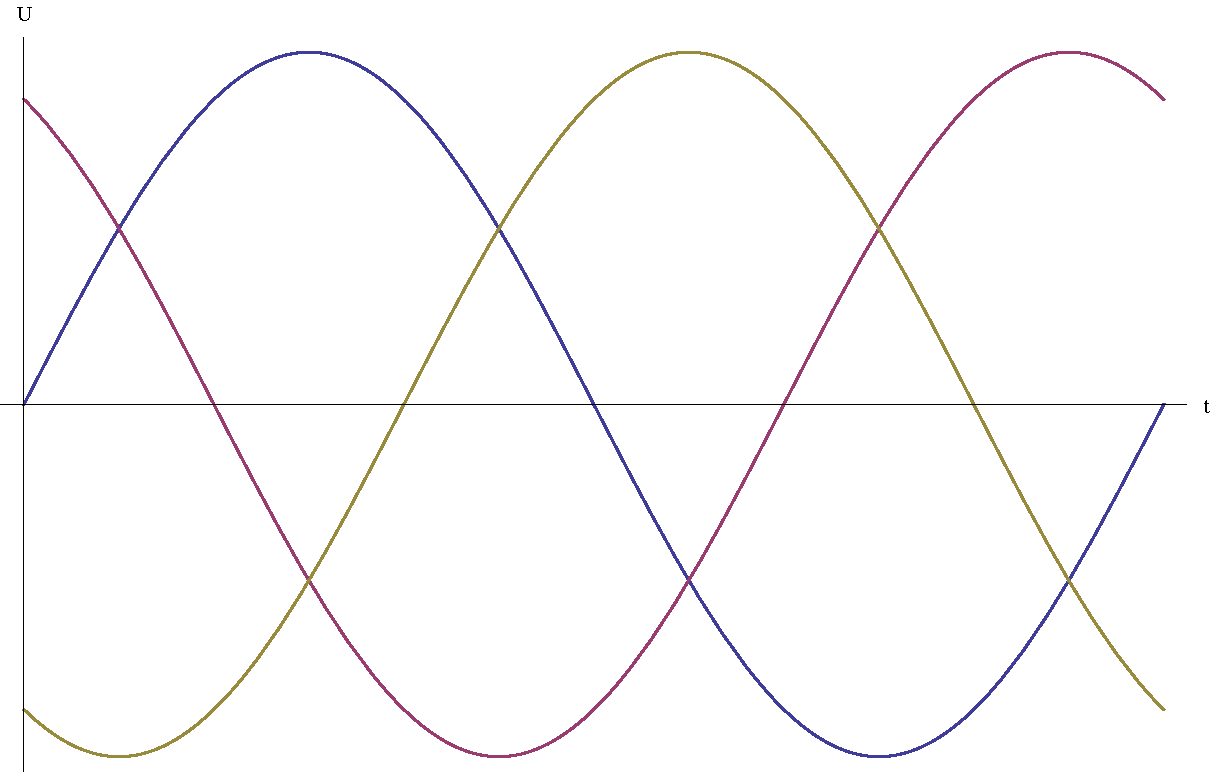
\includegraphics[width=0.5\textwidth]{dreiphasensystem.pdf}
\label{fig:dreiphasensystem}
\caption{Darstellung des Dreiphasensystem mit \textsc{Mathematica}.}
\end{figure}

\section{Einführung Magnetfelder}\label{sec:magnetfelder}

\subsection{Strombelag}\label{sec:strombelag}

Die zeitliche und örtliche Änderung von Magnetfeldern in elektrischen Maschinen wird bestimmt durch die Anordnung stromdurchflossener Leiter und die Art der Speisung \parencite[S.~199]{hofmann2013}.
Die räumliche Verteilung des Stromes wird durch den Strombelag wiedergegeben.
Wenn die Oberfläche eines ferromagnetischen Körpers einen Strombelag $A$ führt, d.\ h.\ wenn eine flächenhafte Strömung vorliegt, liefert das Durchflutungsgesetz

\begin{align}
\oint_{s}{\vec{H}d\vec{s}} = w\cdot I = \Theta \label{durchflutungsgesetz}
\end{align}

$Hds=Ads$, d.\ h.\ $H = A$ bzw.\ $B = \mu A$.
Folgernd existieren neben den Normalkomponenten, $B_n$ und $H_n$ die Tangentialkomponenten $H_t$ und $B_t$ der Feldgrößen.
Die Feldlinien treten nicht mehr senkrecht aus der Randkurve aus, sondern unter einem Winkel $\alpha$.

\begin{align}
\alpha = \arctan(\frac{B_n}{\mu A}) \label{strombelagwinkel}
\end{align}

Der Strombelag wird über dem Umlauf einer Spule bzw.\ Spulengruppe angegeben.

\begin{align}
\Theta(x) = - \int_{x_0}^{x} A(x)dx \label{durchflutung}
\end{align}

damit erhält man durch Differentation den Strombelag $A$

\begin{align}
A(x) = -\partial_x \Theta(x) \label{Strombelag}
\end{align}

mit

\begin{align}
\Theta(x) = \hat{\Theta}(x)\cdot \cos(\frac{\pi}{\tau_p}(x-x_\mu)) \label{adurchflutung}
\end{align}

Nach \ref{durchflutung} ist offensichtlich, dass eine sinusförmige Durchflutungsverteilung nur dann entstehen kann, wenn der Ankerstrombelag ebenfalls sinusförmig, aber um eine Polteilung versetzt ist \parencite[S.~247]{mullerI2005}.

%\begin{figure}[h]
%\centering
%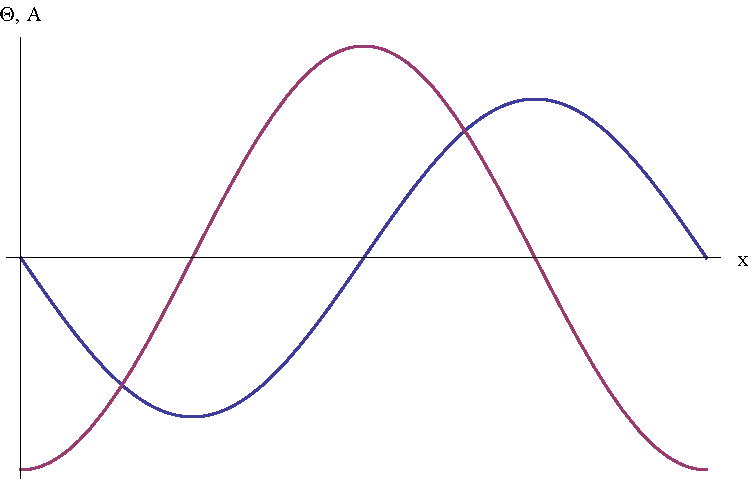
\includegraphics[width=0.5\textwidth]{strombelag.pdf}
%\label{fig:strombelag}
%\caption{Darstellung des sinusförmigen Verlaufs des Strombelags über dem Umlauf.}
%\end{figure}

\section{Allgemeine Grundlagen der Drehstrommaschinen}\label{sec:drehstrommaschinen}

Die Synchron- und Asynchronmaschine besitzen im Ständer denselben Aufbau und erfordern zur Darstellung ihres Verhaltens eine Reihe gleicher physikalischer Begriffe.
Es ist zweckmäßig die Grundlagen der Synchronmaschine in einem eigenen Kapitel zu behandeln.
Dies gilt \insb für den Aufbau der Drehstromwicklungen sowie die Grundlagen zu Beschreibung von umlaufenden Durchflutungen und deren Felder.

\subsection{Drehstromwicklungen}

Der prinzipielle Aufbau einer Drehstromwicklung lässt sich anhand aus den Anforderungen zur Erzeugung einer dreiphasigen Wechselspannung erläutern.
Eine solche Drehspannung erhält man mit einer Anordnung nach \autoref{fig:drehstromwicklung}.
Ein aus Dynamoblechen geschichtetes Ständerblechpacket enthält in Nuten am Bohrungsumfang gleichmäßig verteilte Leiter, die zu drei räumlich verteilten Wicklungssträngen zusammengeschaltet werden \autocite[S.~141]{fischer2009}.
Der Läufer erzeugt ein Gleichfeld, das eine sinusförmige Feldverteilung längst des Luftspaltes aufbaut.
Hat der Läufer eine konstante Drehzahl, so induziert das Feld in den einzelnen Spulen zeitlich sinusförmige Spannungen, die sich innerhalb eines Wicklungsstranges zu einem Wert addieren.
Die Berechnung der Induktion kann über die Allgemeine Beziehung

\begin{align}
u_q = B\cdot l \cdot v
\end{align}

erfolgen.
Sei $d_1$ der Bohrungdurchmesser des Ständerblechpaketes einer $2p$-poligen Maschine, so bezeichnet man den Umfangsanteil

\begin{align}
\tau_p = \frac{d_1 \cdot \pi}{2p}
\end{align}

wieder als Polteilung.
Die Polteilung entspricht der Länder einer Halbwelle der sinusförmigen Flussdichteverteilung im Luftspalt (enspricht einem elektrischen Winkel von $\omega t = 180^{\circ}$.
Bei einer zweipoligen Maschine mit $p=1$ stimmen somit der räumlich mechanische und der elektrische Winkel überein, allgemein gilt die Beziehung \autocite[S.141f.]{fischer2009}

\begin{align}
\gamma_{el} = p\cdot \gamma_{mech}
\end{align}



\begin{figure}[!htb]
\centering
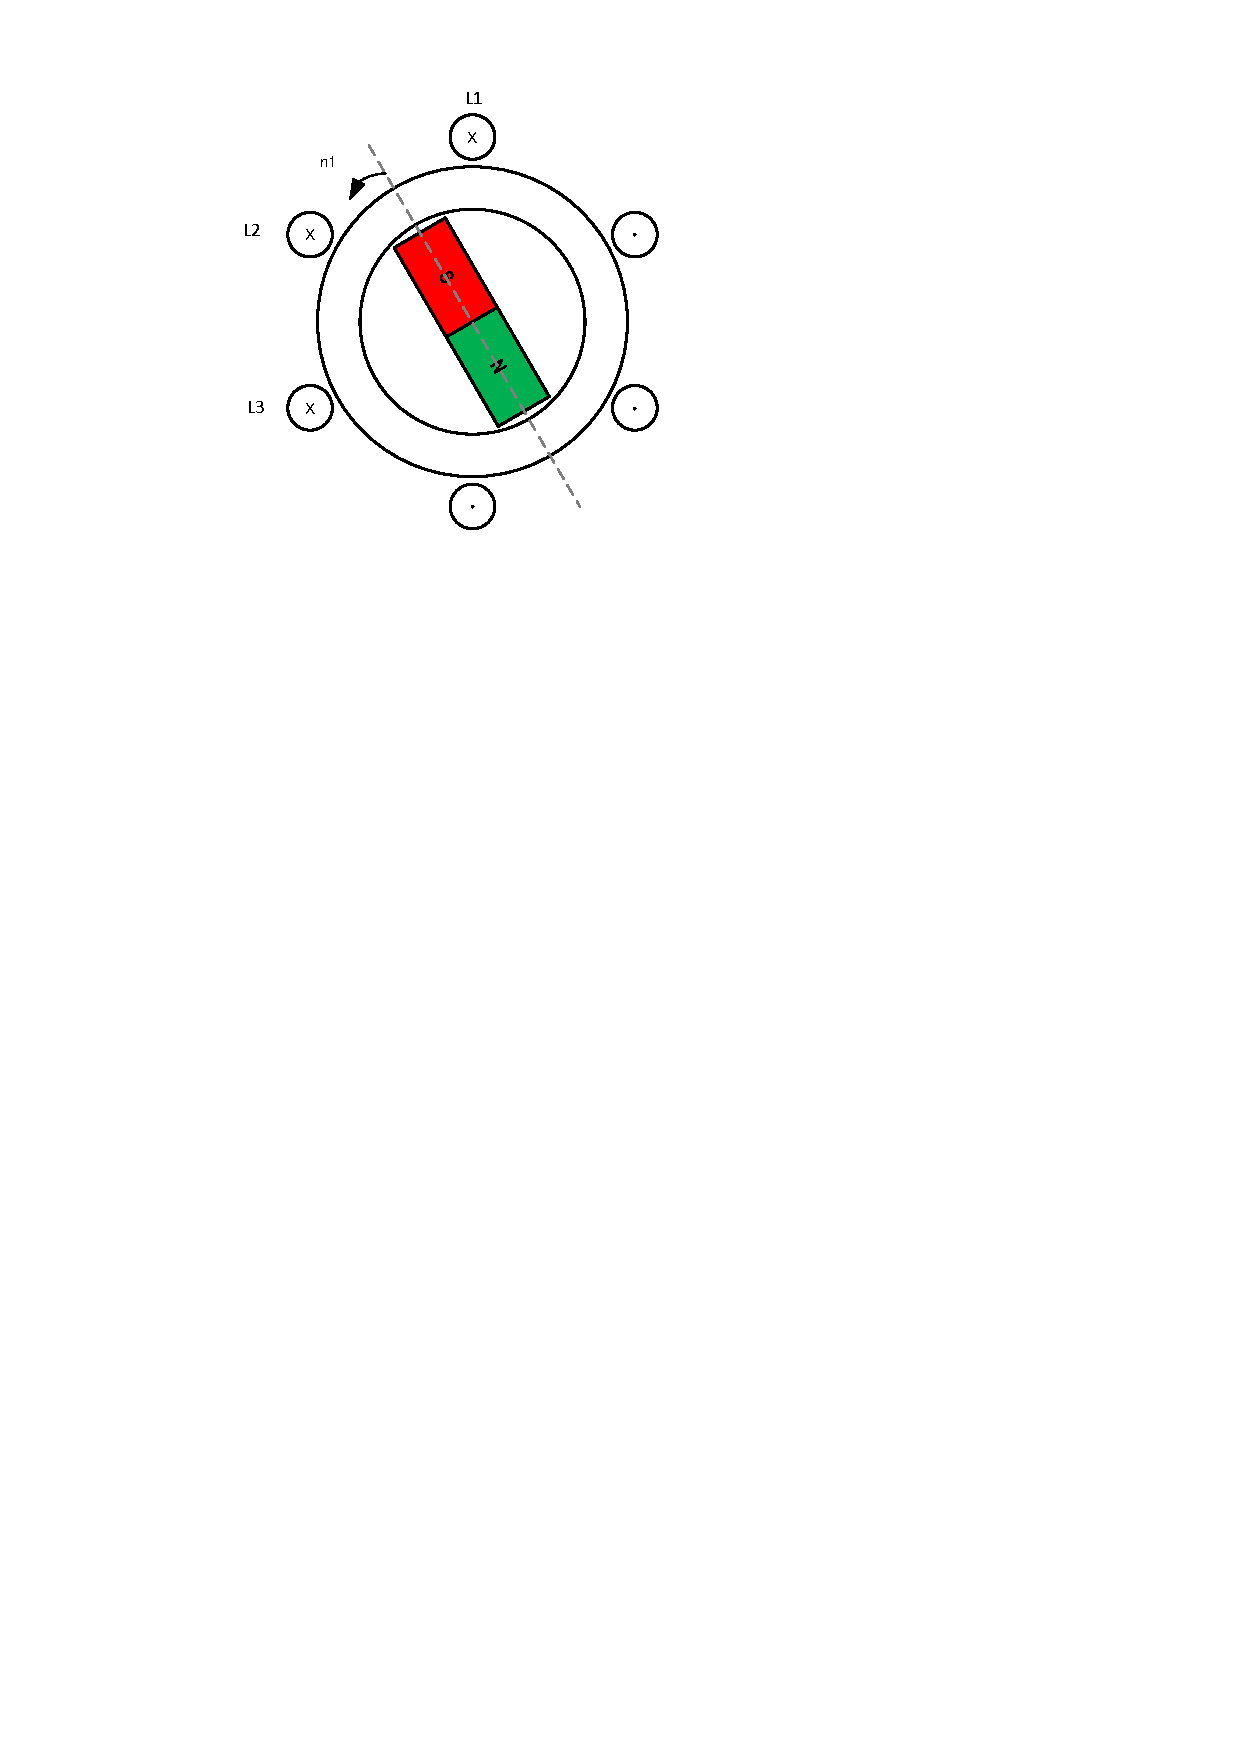
\includegraphics[width=0.5\textwidth]{Visio-synchronmaschine-drehstrom.pdf}
\label{fig:drehstromwicklung}
\caption{Erzeugung einer mehrphasigen Spannung durch ein räumlich sinusförmiges Läuferdrehfeld in Anlehnung an \autocite[S.~141]{fischer2009}}
\end{figure}

\section{Induktivitäten}\label{sec:induktiv}

\section{Einführung Synchronmaschine}\label{sec:synchron}

\paragraph{Historischer Hintergund} Die ersten Synchronmaschinen wurden als Einphasengenerator entwickelt und gebaut, den ersten dreiphasigen Synchrongenerator entwickelten 1887 unabhängig voneinander F.~A.~Haselwander\footnote{Friedrich August Haselwander war ein deutscher Ingenieur, ein Erfinder der Drehstrom-Synchronmaschine und des kompressorlosen Ölmotors.} und C.~S.~Bradley\footnote{Charles Schenk Bradley war ein US-amerikanischer Elektrotechniker, Erfinder und Pionier von frühen Elektromotoren. Er zählt neben F.~A.~Haselwander zu den Begründern des heute im Bereich der elektrischen Energietechnik eingesetzten Dreiphasenwechselstromes.} Bei den Entwicklungen bildeten sich die Bauformen der Schenkelpol- und Vollpolmaschine aus. Die Weiterentwicklung der Synchronmaschine hing stark mit dem Ausbau der Energieversorgung und dem Bedarf von leistungsstärkeren Generatoren zusammen. Unabhängig von der Entwicklung wurden schon sehr früh Synchronmaschinen als Antriebsmaschinen für eine konstante Drehzahlregelung oder einen Phasenbetrieb in der Industrie eingesetzt \autocites[S.~108f.]{ternes2012}[S.~287]{fischer2009}[S.~485f.]{mullerI2005}.

Die gleichstromgespeiste Erregerwicklung ermöglicht es, das Magnetfeld unabhängig vom Netz zu beeinflussen.
Als Spannungsquelle für die Speisung der Erregerwicklung wurden sog.\ Gleichstromerregermaschinen eingesetzt, in der heutigen Zeit werden Wechselspannung mit Hilfe von Leistungselektronischen Schaltungen gespeist.
Um die Schleifringübertragung der Erregerleistung zu umgehen, werden schleifring- bzw.\ bürstenlose Erregersysteme realisiert \autocite[S.~108]{ternes2012}.
Als Motor wurden Drephasen-Synchronmaschinen schon bald für große Leistungen eingesetzt, \zB zum Antrieb von Pumpen und Verdichten \autocite[S.~486]{mullerI2005}.
Der Nachteil ist, dass die Drehzahl durch die Netzfrequenz festgelegt ist.
Die Synchronmaschine arbeitet unabhängig von der Belastung stets mit der durch die Netzfrequenz und die ausgeführte Polpaarzahl festgelegten synchronen Drehzahl.

Heute ist es möglich mit Hilfe eines Frequenzumrichters die Drehzahl der Synchronmaschine zu steuern.
Aus diesem Grund werden größere Gleichstrommaschinen durch drehzahlvariable Synchronmaschinen abgelöst.
Im Bereich kleinerer Leistungen wird anstelle der Gleichstromerregung eine Erregung durch Permanentmagnete eingesetzt.
Dabei verliert man die Beeinflussung des Erregerzustandes über den Erregerstrom, dafür erhält man eine elektrische Maschine die keine elektrische Verbindung zum Läufer erfordert.


\subsection{Beschreibung der Synchronmaschine im dq-Koordinatensystem}

\begin{figure}[!htb]
\centering
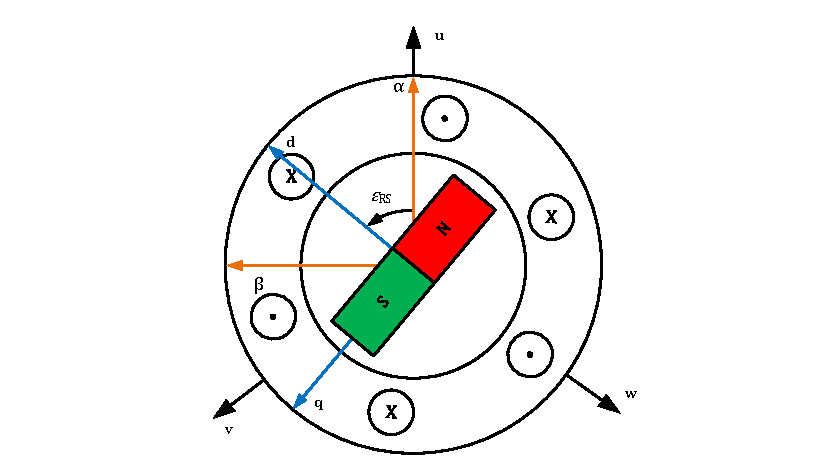
\includegraphics[width=\textwidth]{synchron-dq.pdf}
\label{fig:synchron-dq}
\caption{Darstellung der Synchronmaschine im dq-Koordinatensystem in Anlehnung an \parencite[S.~257]{schroeder2000}.}
\end{figure}

\section{Besonderheiten der Schenkelpolmaschine}\label{sec:schenkelpol}

\section{Permanenterregte Synchronmaschine}\label{sec:pmsm}

\section{Evalurierung der Ersatzschaltbilder für die Regelung}\label{sec:esb}

\begin{figure}[!htb]
\centering
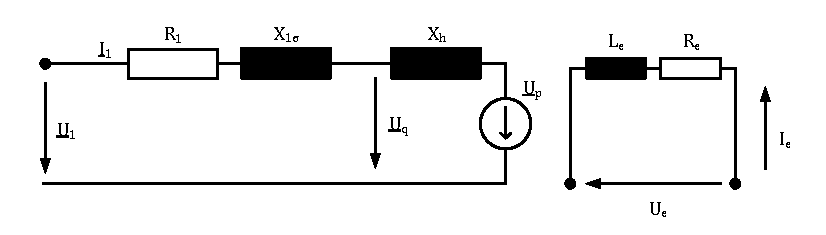
\includegraphics[width=\textwidth]{synchron-esb-kremser2004.pdf}
\label{fig:esb-kremser}
\caption{Ersatzschaltbild der Synchronmaschine nach \parencite[S.~145]{kremser2004}.}
\end{figure}

%%% Local Variables: 
%%% mode: latex
%%% TeX-master: "main"
%%% TeX-open-quote: "\\enquote{"
%%% TeX-close-quote: "}"
%%% LaTeX-csquotes-open-quote: "\\enquote{"
%%% LaTeX-csquotes-close-quote: "}"
%%% End: 


% -*- coding: utf-8 -*-
% !TEX encoding = UTF-8 Unicode
% !TEX root =  main.tex


\chapter{Grundlagen der Vektorregelung}
\label{cha:Grundlagen der Vektorregelung}

%% -- Einführung in die Vektorregelung
In modernen Antriebssystemen ist es häufig unerlässlich, entscheidende Maschinengrößen wie Drehzahl oder Drehmoment auf einen gewünschten Wert einzustellen.
Dabei kamen in der Vergangenheit häufig Gleichstrommaschinen zum Einsatz, welche sich durch gute Regel- und Einstelleigenschaften bei den geforderten Parametern auszeichnen.
Große Fortschritte in den Bereichen der Leistungselektronik und Reglerkomponenten führen dazu, dass Antriebe wesentlich einfacher mit Synchronmaschinen realisiert werden können.
Dabei haben Drehfeldmaschinen, aufgrund fehlender mechanischer Kommutation den Vorteil, dass kein nennenswerter Verschleiß Auftritt.

Entscheidend für den Aufbau einer geregelten PMSM ist die Vektor- bzw. feldorientierte Regelung. 
Die Maschine wird näherungsweise mit sinusförmigen Strömen gespeist. 
Ebenso besitzen alle weiteren auftretenden elektrischen Größen wie Spannungen, Flüsse oder Felder aufgrund ihres Zeitverhaltens annähernd Sinusform \parencite{nuss2010}.	
Die Idee der Vektorregelung ist es , nicht die zeitlichen Momentanwerte der Ströme zu verändern, sondern die erfassten Wechselgrößen in ein zweikomponentiges rotierendes Koordinatensystem zu übertragen.
Dabei beschreibt eine Komponente das Drehmoment, während die andere Komponente die magnetische Flussdichte darstellt.
Diese Größen werden regelungstechnisch verwertet und zurück transformiert.

\section{Raumzeigerdarstellung}
\label{sec:raumzeiger}

Die stationären Zusammenhänge der elektrischen Größen in der Maschine, welche ursächlich aus dem Zusammenhang von $\Psi$ und B herrühren, können zunächst mithilfe komplexer Zeitzeiger beschrieben werden. Dabei lassen sich die Statorströme, $i_\i{u}$, $i_\i{v}$, und $i_\i{w}$ einer Drehfeldmaschine mit idendischer Amplitunde $\hat i_\i{s}$ und Statorkreisfrequenz $\omega_\i{s}$  und der in Abschnitt \ref{subsec:mehrphasensysteme} angeführten Phasenverschiebung $\Delta \varphi = 120^{\circ}$ als:


\begin{align}
	\begin{split}
    i_\i{s,n} = Re\{\underline{i}_\i{s,n}\} = Re\{\underline{\hat i}_\i{s,i}\cdot e^{j\omega_\i{s}t}\} = Re\Bigl\{\hat{i_\i{s}}\cdot e^{j(\omega_\i{s}t+0-(n-1)\cdot\tfrac{2\pi}{3})}\Bigr\}
	\\=\hat{i}_\i{s}\cdot\si{cos}\bigg(\omega_\i{s}t+\varphi_\i{0}-(n-1)\cdot\frac{2\pi}{3}\bigg)~;~mit~n=1,2,3 \label{statorströme} 
\end{split}
\end{align}

mit den komplexen Zeitzeigern

\begin{align}
	\underline{i}_\i{s,n} = \underline{\hat i}_\i{s,n}\cdot e^{j\omega_\i{s}t}~;~mit~n=1,2,3 \label{zeitzeiger}
\end{align}

und den komplexen Amplituden

\begin{align}
	\underline{\hat i}_\i{s,n} = \hat{i_\i{s}}\cdot e^{j(\omega_\i{s}t+0-(n-1)\cdot\tfrac{2\pi}{3})}~;~mit~n=1,2,3 \label{amplituden}
\end{align}

entwickeln. 
Die folgende Abbildung \ref{fig:zeitzeiger} veranschaulicht die vorangegangenen Gleichungen (\ref{statorströme}), (\ref{zeitzeiger}) sowie (\ref{amplituden}) und stellt beispielhaft den Zeitzeiger $i_{s,u}$ dar.

\begin{figure}[h]
	\centering
	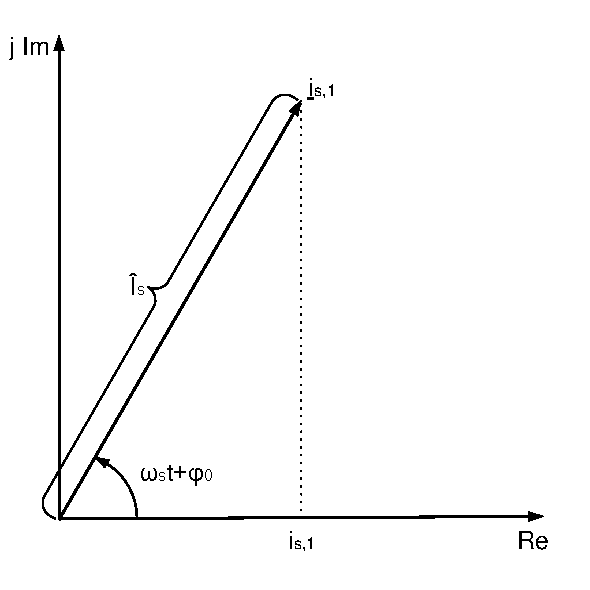
\includegraphics[width=\textwidth]{/vektor/zeitzeiger.pdf}
	\label{fig:zeitzeiger}
	\caption{Beispielhafte Lage eines Zeitzeigers.}
\end{figure}

Da das Ziel darin besteht, den dynamischen Rotationsvorgang einer PMSM zu modellieren, ist die Verwendung eines Zeitzeigers, mit dem nur stationöre Vorgänge beschrieben werden können, nicht angebracht. 
Hier ist es zweckmäßig, einen Operator so zu entwickeln, dass dieser in der Lage ist, dynamische Vorgänge zu beschrieben, ohne dazu Nebenbedingungen wie beispielsweise die Periodizität heranzuziehen. 
Bei der Entwicklung bieten sich die Statorphasenströme $i_\i{s,u}$, $i_\i{s,v}$, und $i_\i{s,w}$ des Dreiphasensystems an.
Diese stehen zu jedem Zeitpunkt zur Verfügung. 
Es sei angemerkt, dass dabei die Nullbedingung erfüllt ist. 
Die Summe der Statorphasenströme muss immer Null sein, was beim Einsatz von Drehfeldmaschinen idr. gegeben ist.
Dadurch ist es auch immer möglich mit Kenntnis zweier Größen auf die Dritte zu schließen, da gilt:

\begin{align}
	i_\i{s,u} + i_\i{s,v} + i_\i{s,w} = 0 
	\label{knotengleichung}
\end{align}


Nun ist der zweikomponentige Zeitzeiger immer um mindestens zwei Momentanwerte erweiterbar. 
Ein hierfür geeigneter Ansatz zur Erzeugung eines Raumzeigers wird in \parencite{nuss2010} gewählt:

\begin{align}
	\underline{i}_\i{s}(t) = \frac{2}{3} \cdot \Bigl\{\underline{i}_\i{s,u}(t) + \underline{i}_\i{s,v}(t)\cdot e^{j\tfrac{2\pi}{3}} + \underline{i}_\i{s,w}(t)\cdot e^{j\tfrac{4\pi}{3}} \Bigr\} \label{statorstromzeiger}
\end{align}

Um jetzt aufzeigen zu können, dass der Ansatz aus Gleichung (\ref{statorstromzeiger}) im stationären Zustand mit dem entsprechenden Statorstromzeitzeiger übereinstimmt und schlussendlich den Raumzeiger zu erzeugen, werden zunächst in Gleichung (\ref{statorstromzeiger}) die Statorstrommomentanwerte aus Gleichung (\ref{statorströme}) eingesetzt.
Dadurch erhält man:

\begin{align}
	\begin{split}
\underline{i}_\i{s}(t) = \frac{2}{3} \cdot \biggl\{\hat{i}_\i{s}\cdot\si{cos}(\omega_\i{s}t+\varphi_{0}) + \hat{i}_\i{s}\cdot\si{cos}\bigg(\omega_\i{s}t+\varphi_{0}-\frac{2\pi}{3}\bigg)\cdot e^{j\tfrac{2\pi}{3}} + \\ \hat{i}_\i{s}\cdot\si{cos}\bigg(\omega_\i{s}t+\varphi_\i{0}-\frac{4\pi}{3}\bigg)\cdot e^{j\tfrac{4\pi}{3}} \biggr\}
\label{zwischen1}
\end{split}
\end{align}

Wird nun die Cosinus-Funktion durch die entsprechende exponentielle Darstellung ersetzt, folgt hieraus:

\begin{align}
	\begin{split}
	\underline{i}_\i{s}(t) = \frac{2}{3} \cdot \hat{i}_\i{s} \cdot \biggl\{ \frac{1}{2} \cdot ( e^{j(\omega_\i{s}t+\varphi_\i{0})} + e^{-j(\omega_\i{s}t+\varphi_\i{0})} ) + \\ \frac{1}{2} \cdot ( e^{j(\omega_\i{s}t+\varphi_\i{0}-\frac{2\pi}{3})} + e^{-j(\omega_\i{s}t+\varphi_\i{0}-\frac{2\pi}{3})})\cdot e^{j\tfrac{2\pi}{3}} + \\ \frac{1}{2} \cdot ( e^{j(\omega_\i{s}t+\varphi_\i{0}-\frac{4\pi}{3})} + e^{-j(\omega_\i{s}t+\varphi_\i{0}-\frac{4\pi}{3})})\cdot e^{j\tfrac{4\pi}{3}}  \biggr\}
	\label{zwischen2}
	\end{split}
\end{align}

Nach ausmultiplizieren der Terme folgt mit $1+e^{j\tfrac{4\pi}{3}}+e^{j\tfrac{8\pi}{3}}=0$ das Ergebnis und somit der Raumzeiger:

\begin{align}
\begin{split}
	\underline{i}_\i{s} = \frac{2}{3} \cdot \hat{i}_\i{s}\cdot\biggl\{ \frac{3}{2} \cdot  e^{j(\omega_\i{s}t+\varphi_\i{0})} + \frac{1}{2} \cdot e^{-j(\omega_\i{s}t+\varphi_\i{0})} \cdot \bigg( 1+e^{j\tfrac{4\pi}{3}}+e^{j\tfrac{8\pi}{3}} \bigg)  \biggr\} = \hat{i}_\i{s} \cdot e^{j(\omega_\i{s}t+\varphi_\i{0})}
	\label{zeigerende}
\end{split}
\end{align}

\newpage

Das Ergebnis der Gleichung (\ref{zeigerende}) entspricht strukturell dem aus Gleichung (\ref{statorströme}) angegebenen Statorstromzeitzeiger. 
Dadurch ist sichergestellt, dass der Ansatz aus Gleichung (\ref{statorstromzeiger}) in der Lage ist als Gesamtzeiger, bestehend aus den Momentanwerten der Statorströme, zu fungieren. 
Die folgende Abbildung \ref{fig:raumzeigermaschine} zeigt zur Veranschaulichung eine zweipolige Drehfeldmaschine mit zugehörigem Zeigerdiagramm, welches den Statorstromraumzeiger beinhaltet. 

\begin{figure}[h]
	\centering
	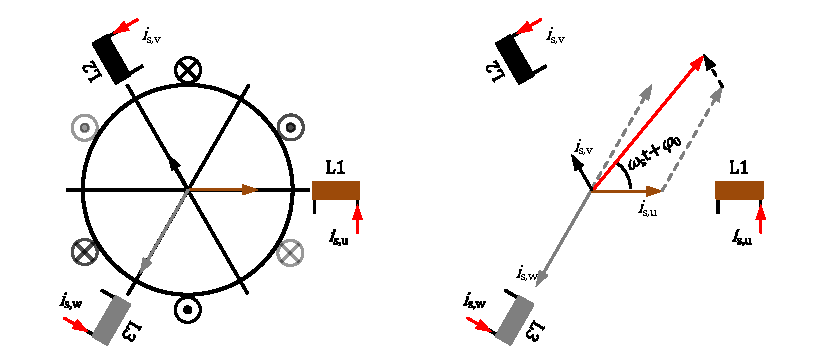
\includegraphics[width=\textwidth]{/vektor/raumzeigermaschine.pdf}
	\label{fig:raumzeigermaschine}
	\caption{zweipolige Drehfeldmaschine}
\end{figure}


Mit der Einführung des Raumzeigers ist die theoretische Grundlage dafür geschaffen, die PMSM feldorientiert zu regeln.
Da sich, wie eingangs beschrieben, alle Größen in der Drehfeldmaschine näherungsweise sinusförmig verhalten, ist die Stromraumzeigerdarstellung aus Gleichung (\ref{statorstromzeiger}) für alle anderen dreiphasigen Größen als allgemeine Raumzeigerdarstellung definierbar.

\begin{align}
	\underline{a}(t) = \frac{2}{3} \cdot \Bigl\{\underline{a}_\i{u}(t) + \underline{a}_\i{v}(t)\cdot e^{j\tfrac{2\pi}{3}} + \underline{a}_\i{w}(t)\cdot e^{j\tfrac{4\pi}{3}} \Bigr\} \label{raumzeigerdefinition}
\end{align}

Im Folgenden werden die in der Praxis benötigten Transformationsvorschriften erläutert, welche das Wechseln zwischen Phasen- und Raumzeigergrößen erlauben.


\section{Beschreibung in $\alpha$-$\beta$-Koordinatensystem}\label{sec:clark}

Als Grundlage für das Wechseln zwischen Phasen- und Raumzeigergrößen dient zunächst die Definition aus Gleichung (\ref{raumzeigerdefinition}). Die Definitionsgleichung lässt sich in Real- und Imaginärteil aufspalten. Es kommt so zu folgender Aufteilung:

\begin{align}
	Re~{\underline{a}(t)} = \frac{2}{3} \cdot \Bigl\{ a_{u}(t) + a_{v}(t) \cdot\cos{\frac{2 \pi}{3}} + a_{w}(t) \cdot\cos{\frac{4 \pi}{3}} \Bigr\}
	\label{realteil}
\end{align}

\begin{align}
	Im~{\underline{a}(t)} = \frac{2}{3} \cdot \Bigl\{a_{v}(t)\cdot\sin{\frac{2 \pi}{3}} + a_{w}(t) \cdot\sin{\frac{4 \pi}{3}} \Bigr\}
	\label{imaginärteil}
\end{align}

In Zusammenhang mit der Clarke-Transformationsvorschrift ist es üblich, den Realteil in $\alpha$-Koordinaten und den Imaginärteil als $\beta$-Koordinaten auszudrücken. 
Daher ist die Clarke-Transformation im deutschsprachigen Bereich auch $\alpha$-$\beta$-Transformation bekannt.
Um im Weiteren die in der Praxis notwendige Transformationsmatrix zu erhalten, werden die trigonometrischen Ausdrücke numerisch dargestellt. 
Aus den Gleichungen (\ref{realteil}) und (\ref{imaginärteil}) folgt somit:

\begin{align}
	a_{\alpha}(t) = \frac{2}{3} \cdot \Bigl\{ a_{u}(t) - \frac{1}{2} \cdot a_{v}(t) - \frac{1}{2} \cdot a_{w}  \Bigr\}
	\label{alpha}
\end{align}

\begin{align}
	a_{\beta}(t) = \frac{2}{3} \cdot \Bigl\{\frac{\sqrt{3}}{2} \cdot a_{v}(t) - \frac{\sqrt{3}}{2} \cdot a_{w}  \Bigr\}
	\label{beta}
\end{align}

Der entstandene Raumzeiger in  $\alpha$-$\beta$-Koordinaten ist in allgemeiner Form als 

\begin{align}
	\underline{a}(t) = a_{\alpha}(t) +j a_{\beta}(t)
	\label{raumzeigeralphabeta}
\end{align}

darstellbar. Um die $\alpha$- und $\beta$-Komponente des entstandenen Raumzeigers besser nachvollziehen zu können, zeigt die Abbildung \ref{fig:alphabetakoordinaten} eine beispielhafte Lage des Zeigers in $\alpha$-$\beta$-Koordinaten.
\newpage

\begin{figure}[h]
	\centering
	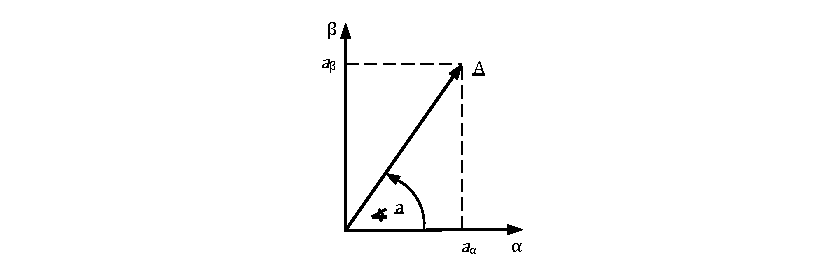
\includegraphics[width=\textwidth]{/vektor/alphabetakoordinaten.pdf}
	\label{fig:alphabetakoordinaten}
	\caption{Lage des Raumzeigers im $\alpha$-$\beta$-Koordinatensystem.}
\end{figure}

Nachdem sich der Raumzeiger im neuern Koordinatensystem darstellen lässt, ist es nun entscheidend, eine mathematische Transformationsvorschrift aufzustellen, die sich an Gleichungen (\ref{alpha}) und (\ref{beta}) orientiert. 
Übertragen in eine Matrix lautet die Transformation und Transformationsmatrix $\underline{T}^{\prime}$:

\begin{align}
	\begin{bmatrix}
	a_{\alpha} \\
	a_{\beta} 
	\end{bmatrix}
	=\frac{2}{3}\cdot\underline{T}^{\prime}
	\begin{bmatrix}
	a_{u} \\
	a_{v} \\
	a_{w}
	\end{bmatrix}
	\label{clarkevektor}
\end{align}

mit der Transformationsmatrix

\begin{align}
	\underline{T}^{\prime} = 
	\begin{bmatrix}
		1 & -\frac{1}{2} & -\frac{1}{2}  \\
		0 & ~~\frac{\sqrt{3}}{2} & ~~\frac{\sqrt{3}}{2}
	\end{bmatrix}
	\label{clarkematrix}
\end{align}

Mit dieser Matrix ist es möglich, die dynamische Drehfeldgößen eines dreiphasigen Systems auf zwei Größen zu reduzieren sowie Momentanwerte und Amplitude in einem Raumzeiger darzustellen.
Der Faktor $\frac{2}{3}$ normiert dabei $a_{\alpha}$ und $a_{\beta}$ auf den Betrag der entsprechenden Eingangsgrößen.

Für eine Regelung fehlt eine Rücktransvormationsvorschrift, mit deren Hilfe die $\alpha$- und $\beta$-Komponente wieder in ein Dreiphasensystem gebracht werden kann.
Die inverse Matrix bildet sich aus Gleichung (\ref{clarkematrix}). 
Da es sich hier aber um eine nichtquadratische Matrix handelt, ist diese zunächst nicht invertierbar.
Folglich muss die Matrix um eine Eingangsgröße erweitert werden.
Dabei bietet sich die Nullbedingung des Systems an.
Bindet man die Knotengleichung aus Gleichung (\ref{knotengleichung}) in Gleichung (\ref{clarkematrix}) ein, folgt für die vektorielle Transformationsbeziehung:

\begin{align}
	\begin{bmatrix}
		a_{\alpha} \\
		a_{\beta} \\
		a_{0}
	\end{bmatrix}
	=\underline{T}\cdot 
	\begin{bmatrix}
		a_{u} \\
		a_{v} \\
		a_{w}
	\end{bmatrix}
	\label{clarkevektornull}
	\end{align}

mit der Transformationsmatrix

\begin{align}
	\underline{T} =
	\begin{bmatrix}
		1 & -\frac{1}{2} & -\frac{1}{2}  \\
		0 & ~~\frac{\sqrt{3}}{2} & ~-\frac{\sqrt{3}}{2} \\
		\frac{1}{2} & ~~\frac{1}{2} & ~~\frac{1}{2}
	\end{bmatrix}
	\label{clarkematrixnull}
\end{align} 

Die auf diese Art entstandene quadratische Matrix ist eindeutig invertierbar.
Daher folgt für

\begin{align}
	\begin{bmatrix}
	a_{u} \\
	a_{v} \\
	a_{w}
	\end{bmatrix}
	=\underline{T}^{-1}\cdot 
	\begin{bmatrix}
	a_{\alpha} \\
	a_{\beta} \\
	a_{0}
	\end{bmatrix}
	\label{inverseclarkevektornull}
\end{align}

die inverse Transformationsmatrix

\begin{align}
	\underline{T}^{-1} =
	\begin{bmatrix}
		~~1 & 0 & 1  \\
		-\frac{1}{2} & -\frac{\sqrt{3}}{2} & 1 \\
		~-\frac{1}{2} & -\frac{\sqrt{3}}{2} & 1
	\end{bmatrix}
	\label{inverseclarkematrixnull}
\end{align}

Für die Praxisanwendung reicht die vereinfachte inverse Clarke-Transformation mit der Beziehung

\begin{align}
	\begin{bmatrix}
		a_{u} \\
		a_{v} \\
		a_{w}
	\end{bmatrix}
	=\underline{T}^{-1}\cdot 
	\begin{bmatrix}
		a_{\alpha} \\
		a_{\beta} \\
	\end{bmatrix}
	\label{inverseclarkevektornulleinfach}
\end{align}
 
 und der Transformationsmatrix 
 
 \begin{align}
 	\underline{T}^{-1} =
 	\begin{bmatrix}
 		~~1 & 0   \\
 		-\frac{1}{2} & -\frac{\sqrt{3}}{2}  \\
 		~-\frac{1}{2} & -\frac{\sqrt{3}}{2} 
 	\end{bmatrix}
 	\label{inverseclarkematrixnulleinfach}
 \end{align}
 
 aus. 
 Da die Nullkomponente der Phasengröße aufgrund der symmetrischen Belastung null ist, kann auch $a_{0}$ null gesetzt werden, was dem Wegfall der letzten Spalte von ${\underline{T}^{-1}}$ entspricht. Zusammgefassend ist die Transformation in der folgenden Abbildung \ref{fig:clarktransformationdiagramm} erkennbar.
 
 \begin{figure}[h]
 	\centering
 	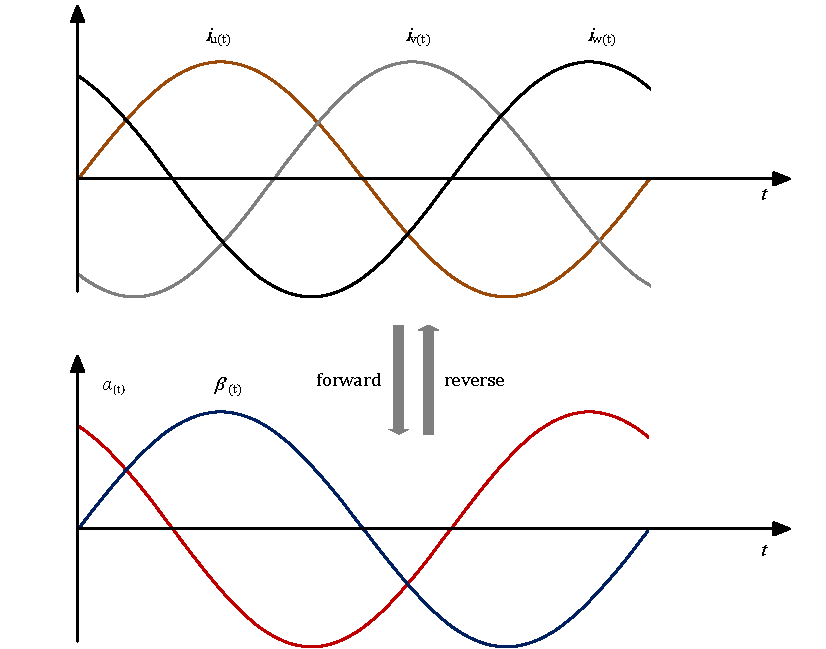
\includegraphics[width=\textwidth]{/vektor/clarktransformationdiagramm.pdf}
 	\label{fig:clarktransformationdiagramm}
 	\caption{Clarke-Transformation}
 \end{figure}
 

\section{Beschreibung in rotorfesten d-q-Koordinatensystem}\label{sec:park}

Für die Regelung von Drehfeldmaschinen hat es sich als praktikabel herausgestellt, die Beschreibung des im Vorfeld beschriebenen ortsfesten Koordinatensystems in ein, mit der Winkelgeschwindigkeit des Rotors, rotierendes Koordinatensystem zu überführen. 
Daher wird die Darstellung auch rotorfest genannt. 
Die Vorteile dieser Koordinatenbeschreibung liegen zum einen in einer einfacheren Darstellbarkeit elektrophysikalischer Zusammenhänge und zum anderen daran, dass die Raumzeigergrößen näherungsweise Gleichgrößen sind.
Dadurch lassen sich klassische Regelverfahren auf die Maschine anwenden.
Das Regelverhalten ähnelt dem der Gleichstrommaschine, welche sich durch eine gute Regelbarkeit auszeichnet. 
Für die folgende Park-Transformation dient die zuvor durchgeführte Clarke-Transformation als Grundlage. 
Zur Verdeutlichung der Transformationsvorschriften dient die nachfolgende Abbildung \ref{fig:dqkoordinaten} am Beispiel eines Statorstromraumzeigers.

\begin{figure}[h]
	\centering
	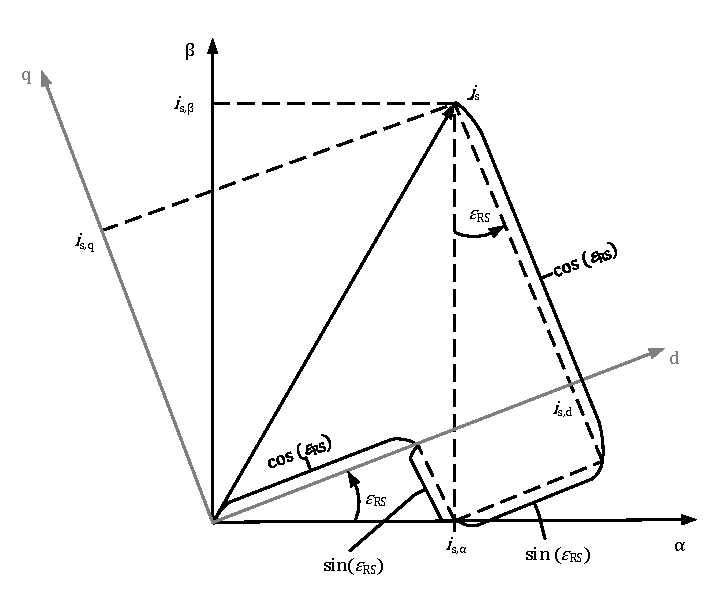
\includegraphics[width=\textwidth]{/vektor/dqkoordinaten.pdf}
	\label{fig:dqkoordinaten}
	\caption{Zusammenhang von $\alpha$-$\beta$-Koordinaten und d-q-Koordinaten}
\end{figure}


Hier ist neben dem ortsfesten $\alpha$-$\beta$-Koordinatensystem auch das rotierende Koordinatensystem erkennbar. 
Das rotierende System wird als d-q-Koordinatensystem bezeichnet, wobei $d$ für direct axis und $q$ für quadrature axis steht.
Der für die Transformation entscheidende Winkel ist hier mit $\varepsilon_\i{RS}$ gekennzeichnet.
Mit Hilfe der Abbildung lässt sich nun die Transformationsbeziehung zwischen $\alpha$-$\beta$-Koordinaten und d-q-Koordinaten aufstellen.

\begin{align}
	\begin{bmatrix}
		a_\i{d} \\
		a_\i{q} 
	\end{bmatrix}
	=\underline{T}{^\prime}\cdot 
	\begin{bmatrix}
		a_{\alpha} \\
		a_{\beta}
	\end{bmatrix}
	\label{parkvektor}
\end{align}

Die Transformationsmatrix lautet dann

\begin{align}
	\underline{T}{^\prime} =
	\begin{bmatrix}
		~~~\cos({\varepsilon_\i{RS}}) & \sin({\varepsilon_\i{RS}}) \\
		-\sin({\varepsilon_\i{RS}}) & \cos({\varepsilon_\i{RS}})
	\end{bmatrix}
	\label{parkmatrix}
\end{align}

Da die Matrix eine quadratische ist, kann diese ohne weiteres invertiert werden.
Die Rücktransformation von d-q-Koordinaten in $\alpha$-$\beta$-Koordinaten ist für die Regelung ebenfalls von entscheidender Bedeutung, um aus dem rotierenden Raumzeiger im letzten Schritt wieder die drei Phasengrößen zu erhalten. 
Es gilt für die Rücktransformation also die Beziehung

\begin{align}
	\begin{bmatrix}
		a_{\alpha} \\
		a_{\beta}
	\end{bmatrix}
	=\underline{T}^{-1}\cdot 
	\begin{bmatrix}
		a_\i{d} \\
		a_\i{q} 
	\end{bmatrix}
	\label{parkvektorinvers}
\end{align}

mit der Transformationsmatrix

\begin{align}
	\underline{T}^{-1} =
	\begin{bmatrix}
		\cos({\varepsilon_\i{RS}}) & -\sin({\varepsilon_\i{RS}}) \\
		\sin({\varepsilon_\i{RS}}) & ~~~\cos({\varepsilon_\i{RS}})
	\end{bmatrix}
	\label{parkmatrixinvers}
\end{align}

Dieser Transformationsschritt ist der Abbildung \ref{fig:parktransformationdiagramm} zu entnehmen.


\begin{figure}[h]
	\centering
	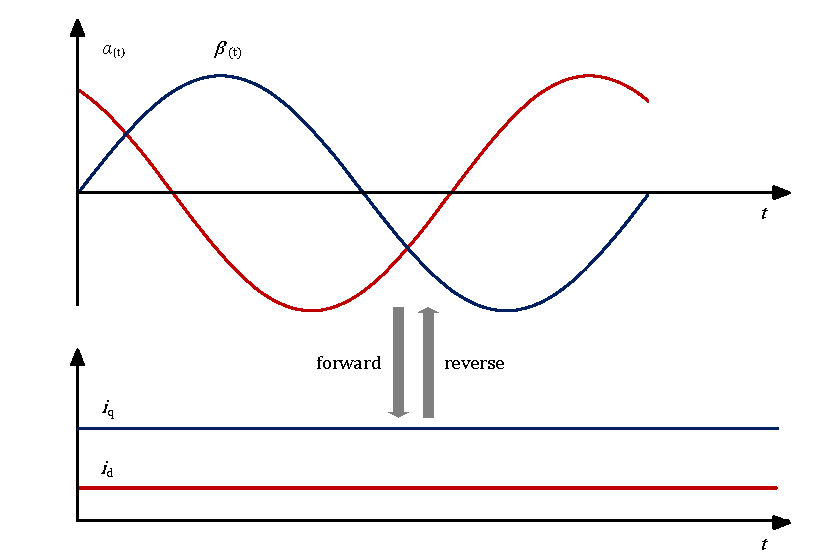
\includegraphics[width=\textwidth]{/vektor/parktransformationdiagramm.pdf}
	\label{fig:parktransformationdiagramm}
	\caption{Park Transformation}
\end{figure}
i
\newpage

\section{Signalflussplan der Koordinatentransformationen}\label{sec:signalflussplan}

In diesem Abschnitt wird mit Hilfe der Transformationsvorschriften aus den vorherigen Abschnitten \ref{sec:clark} und \ref{sec:park} ein Signalflussplan entwickelt.
Dieser Plan soll im praktischen Teil in das Simulationsmodell integriert werden können.
Zur einfacheren Darstellung der Clarke- und Park-Transformation werden zunächst die benötigten Signalflussbilder entwickelt.

\begin{figure}[h]
	\centering
	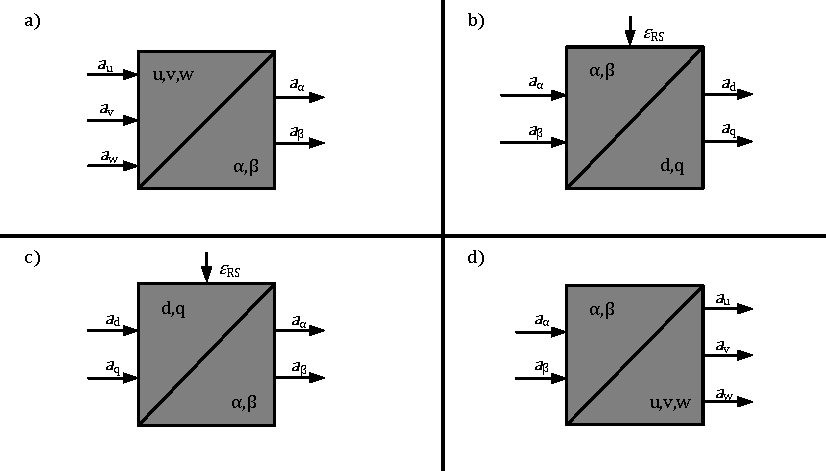
\includegraphics[width=\textwidth]{/vektor/blockbildclarkeparkkomplett.pdf}
	\label{fig:blockbildclarkeparkkomplett}
	\caption{Blockschaltbilder der Transformationen}
\end{figure}

In der Abbildung \ref{fig:blockbildclarkeparkkomplett} a) ist das Blockbild der Clarke-Transformation und in Abbildung \ref{fig:blockbildclarkeparkkomplett} b) die Park-Transformation dargestellt. 
Bei der Parktransformation wird der Winkel $\varepsilon_\i{RS}$, um den das $\alpha$-$\beta$-Koordinatensystem zum d-q-System verschoben ist, zugeführt.
Die entsprechenden Rücktransformationen sind in Abbildung \ref{fig:blockbildclarkeparkkomplett} c) und Abbildung \ref{fig:blockbildclarkeparkkomplett} d) der Grafik veranschaulicht.

Innerhalb des Reglermodells werden die Hin- und Rücktransformationen direkt aufeinander folgen. Daher sind in der nachstehenden Abbildung \ref{fig:blockbildinverseclarkeparkkomplett} die Clarke-Park-Transformation, sowie die Park-Clarke-Transformation als zusammenhängendes Blockbild mit den Stromkomponenten aufgezeigt.
\newpage

\begin{figure}[h]
	\centering
	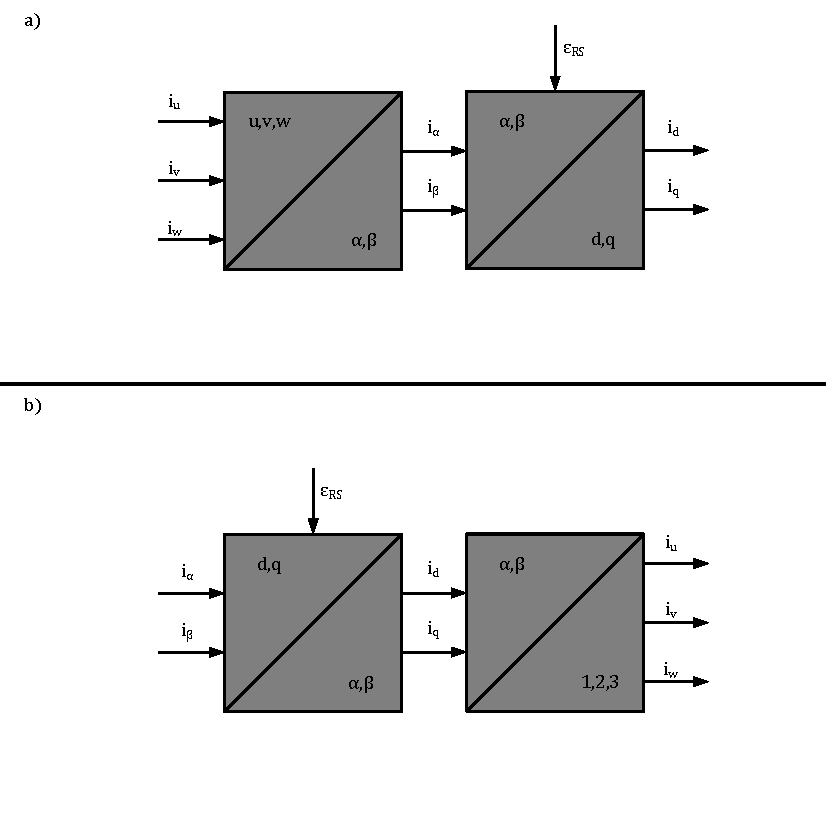
\includegraphics[width=\textwidth]{/vektor/blockbildinverseclarkeparkkomplett.pdf}
	\label{fig:blockbildinverseclarkeparkkomplett}
	\caption{Blockschaltbilder der Transformationen}
\end{figure}

Mit Hilfe der Blockbilder kann jetzt die sowohl die vollständige Hintransformation eines Dreiphasensystems in ein rototorisches, zweikomponentiges Bezugsystem, als auch die entsprechende Rücktransformation, als Signalflussbild skizziert werden.





 
%%% Local Variables: 
%%% mode: latex
%%% TeX-master: "main"
%%% TeX-open-quote: "\\enquote{"
%%% TeX-close-quote: "}"
%%% LaTeX-csquotes-open-quote: "\\enquote{"
%%% LaTeX-csquotes-close-quote: "}"
%%% End: 

% -*- coding: utf-8 -*-
% !TEX encoding = UTF-8 Unicode
% !TEX root =  main.tex

\chapter{Modellbasierte Implementierung der Vektorregelung}
\label{cha:regelungpmsm}

Die Einführung in das Kapitel stellt dem Leser zunächst eine grundlegende Einführung in die Simulationstechniken und dem Anwenderprogramm Simulink dar.
Simulink ist ein Programm, welches mit MATLAB gekoppelt ist, in Simulink kann der Anwender Simulationen durchführen.
Aufgrund der Komplexität von Simulink soll an dieser Stelle nicht weiter auf die Toolboxen eingeganen werden.
Somit erhalten auch Leser ohne Erfahrungen mit dem Softwarepaket, die zum weiteren Verständnis der Arbeit benötigten Grundkenntnisse.
Der Vorteil bei der Nutzung von MATLAB basiert zum einen darauf, dass die Software etablierter Quasistandard in der Industrie und an Hochschulen ist und zum anderen auf der Benutzerfreundlichkeit bei der Durchführung von Projektarbeiten \autocite{scherf2010}.
Dem versierten Anwender der Software sei geraten, diesen Abschnitt zu überspringen.

\section{Simulation von Systemen}\label{sec:simulation}

Simulationen sind heute unverzichtbar bei der Entwicklung und Optimierung von Systemen und der Erforschung von Zusammenhängen komplexer Systeme und Prozesse \autocite{brychta}.
Die meist umfangreichen Prozesse und Systeme werden dazu in Modellen nachgebildet.
Dieses Verfahren eignet sich gut zur Analyse der Systemeigenschaften.
Dabei können die eingesetzten Simulationsmittel unterschiedlich ausfallen.

\begin{enumerate}
	\item Das System wird maßstäblich oder stark vereinfacht mit den wesentlichen Komponenten aufgebaut.
	\item Das System wird durch ein anderes physikalisches Modell nachgebildet.
	\item Das System wird durch ein mathematisches Modell beschrieben.
\end{enumerate}

Bei umfangreichen Simulationen bietet es sich an, das System in \enquote{Subsysteme} zu unterteilen (s.~h.~Abbildung~\ref{fig:subsysteme}), so dass die Modellierung mit Simulink übersichtlicher wird.
Der Vorteil gegenüber der konventionellen Modellierung von umfangreichen System, ist es, dass Fehler früher erkannt und einzelne Systeme auf physikalische Richtigkeit geprüft werden können.

\begin{figure}[h!]
	\centering
	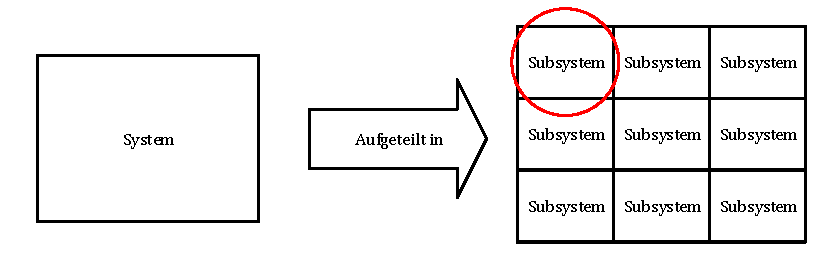
\includegraphics{/simulink/subsysteme.pdf}
	\label{fig:subsysteme}
	\caption{Semantische Abbildung zur Unterteilung eines Systemes in Subsysteme.}
\end{figure}

Das eingekreiste System kann so isoliert und gekapselt beschrieben werden.
Dazu sind die Abhängigkeiten zwischen benachbarten Subsytemen zu erfassen und bei der Kapselung geeignet zu verwerten.
Auch Subsysteme lassen sich in weitere Subsysteme zerlegen (s.~h.~Abbildung~\ref{fig:subsubsysteme}).

\begin{figure}[h!]
	\centering
	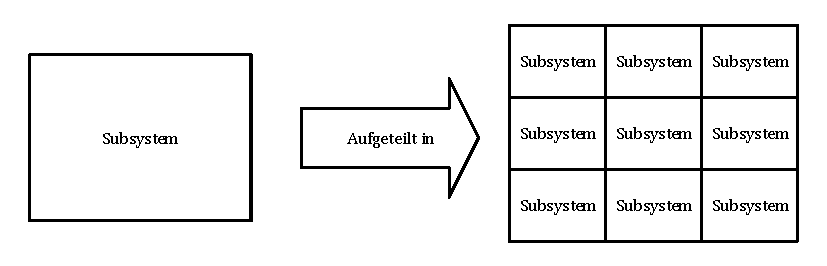
\includegraphics{/simulink/subsubsystem.pdf}
	\label{fig:subsubsysteme}
	\caption{Semantische Abbildung zur Unterteilung eines Subsystems in weitere Subsysteme.}
\end{figure}

Bei der Modellierung sollte auf die Übersichtlichkeit der Systeme geachtet werden.

\section{Einführung in Simulink}\label{sec:simulink}

MATLAB/Simulink ist vom Softwarehersteller \glqq{The Mathworks}\grqq~entwickelt worden.
Zu den Einsatzgebieten der Software zählen hauptsächlich Modellierung und Simulation technischer und physikalischer Systeme. 
MATLAB ist dabei die Kernsoftware, welche sich mit vielen Toolboxen ergänzen lässt. 
Der Name MATLAB wurde dabei von "MATrix LABoratory" abgeleitet.
Vor der Simulation eines technischen Prozesses steht die Modellbildung, welche in den vorangegangenen Kapiteln durchgeführt wurde.
Dazu sind die nötigen physikalischen Gesetzmäßigkeiten zur Beschreibung der Maschine und Regelung genutzt worden.
Als Ergebnis der Modellbildung werden nun die Differentialgleichungen, Verknüpfungen und Zusammenhänge innerhalb von Simulink zu einem geschlossen Simulationsmodell verbunden. 
Der Aufbau von den Systemen findet in Simulink mit Hilfe von Blockbildern statt, welche mit Signalflusspfeilen zu einem Signalflussplan kombiniert werden. 
Entscheidend für die Simulation von dynamischen Systemen ist die Lösung von mathematischen Zusammenhängen, insbesondere von Differentialgleichungen. 

\subsection{Simulationsbeispiel: Das mathematische Pendel}

Zur Modellbildung und Simulation eines dynamischen Fadenpendels sei zunächst die folgende Abbildung \ref{fig:pendel} gegeben:

\begin{figure}[h]
	\centering
	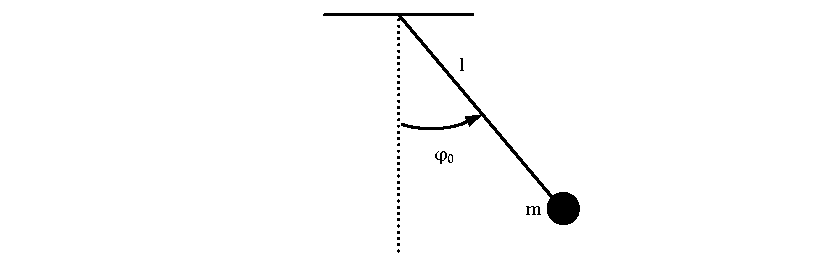
\includegraphics{/regelung/pendel.pdf}
	\label{fig:pendel}
	\caption{Fadenpendel}
\end{figure}

Er gelten folgende Momente:

\begin{center}
	\begin{tabular}{ll}
		\toprule
		Bezeichnung:				&	Mathematisches Modell: \\
		\midrule
		Rückstellmoment				&	$F_\i{Z} = m \cdot g \cdot \si{sin}(\varphi) \label{rueckstellmoment}$ \\
		Beschleunigungsmoment		&	$F_\i{B} = J \cdot \varphi = m \cdot l^{2} \cdot \ddot\varphi\label{beschleunigungsmoment} $ \\
		Reibungsmoment				&	$F_\i{R} = d \cdot l^{2} \cdot \dot\varphi\label{reibungsmoment} $ \\
		Summe aller Kräfte			&	$\sum F = 0 \label{momentengleichgewicht} $ \\
		\bottomrule 
	\end{tabular}
\end{center}

Die Bewegung des Pendels wird mit folgenden Werten simuliert:

\begin{center}
	\begin{tabular}{ll}
		\toprule
		Physikalische Bezeichnung:	& Wert: \\
		\midrule
		m		& \SI{2,3}{kg} \\
		d		& \SI{0,2}{Nms} \\
		l		& \SI{1,1}{m} \\
		g		& \SI{9,81}{m/s^2}\\
		$\varphi$ & \SI{40}{^\circ}\\
		\bottomrule
	\end{tabular}
\end{center}

Als nächster Schritt werden die physikalischen Systembeschreibungen in einer Gesamtformel zusammengefasst. 

\begin{align}
	\sum M = M_\i{R} + M_\i{B} + M_\i{Reib} = 0
	\label{momentengleichgewichtgesamt} 
\end{align}

\begin{align}
	\sum M = m \cdot g \cdot \si{sin}(\varphi) + J \cdot \varphi = m \cdot l^{2} \cdot \ddot\varphi + d \cdot l^{2} \cdot \dot\varphi = 0
	\label{momentengleichgewichtgesamt2} 
\end{align}

Wird nun die Differentialgleichung \ref{momentengleichgewichtgesamt2} nach der höchsten Ableitung $\ddot\varphi$ umgestellt, ergibt sich:

\begin{align}
	\ddot\varphi = -\dot\varphi \cdot \tfrac{\i{d}}{\i{m}} - \tfrac{\i{g}}{\i{l}} \cdot \si{sin}(\varphi)
	\label{diffgleichung} 
\end{align}

An dieser Stelle ist die Modellbildung abgeschlossen. Jetzt können die Werte in MATLAB/Simulink  verarbeitet werden.
Hier werden zuerst in der MATLAB-Umgebung Variablen mit den vorgegebenen Werten parametrisiert.

%\begin{figure}[h]
%	\centering
%	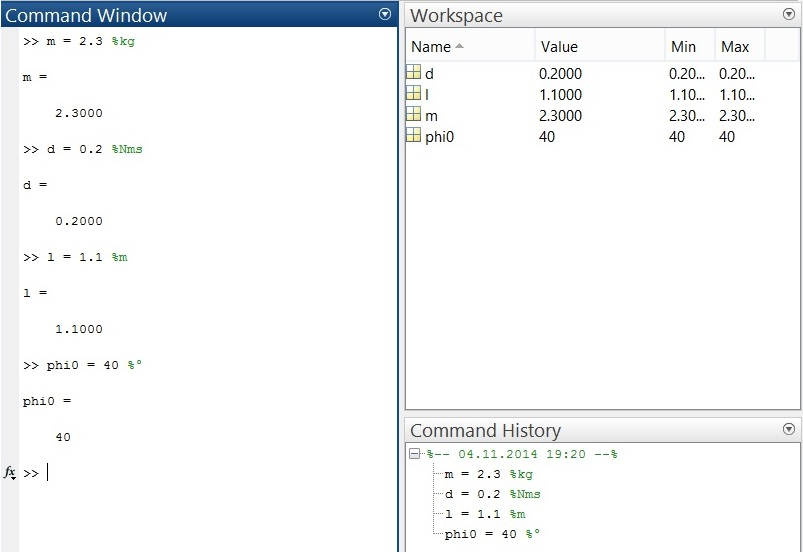
\includegraphics[width=\textwidth]{/regelung/matlab1.jpg}
%	\label{fig:matlab1}
%	\caption{Variablen in Matlab-Umgebung}
%\end{figure}

Anschließend kann in der Simulink-Umgebung das Modell entsprechend \ref{momentengleichgewichtgesamt2} aufgebaut werden.

\begin{figure}[h]
	\centering
	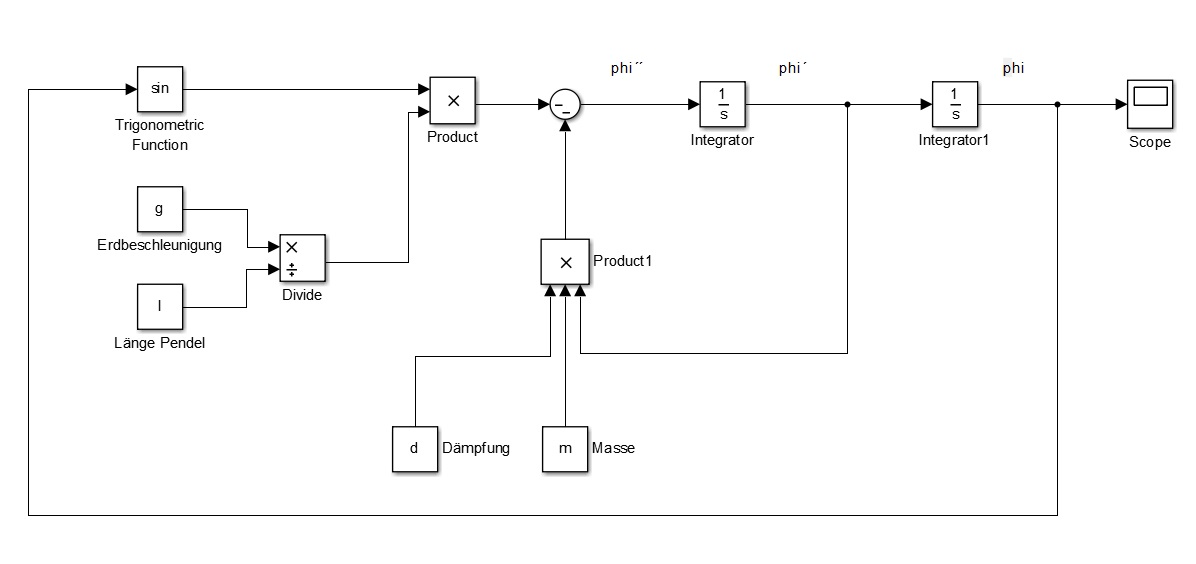
\includegraphics[width=\textwidth]{/regelung/matlab2.jpg}
	\label{fig:matlab2}
	\caption{fertiges Modell in Simulink}
\end{figure}

Mit Hilfe dieser Blöcke lassen sich  $\dot{\varphi}$ und $\varphi$ erzeugen.
Die Simulink Bibliothek bietet eine Vielzahl von mathematischen Operatoren in Form von Blockbildern.
Mit Hilfe dieser Blöcke und der Signalflusspfeile lässt sich die Gleichung in das Simulationsmodell übertragen.
Ist das Modell aufgebaut, werden die Simulationsparameter ausgewählt. 
Simulink arbeitet numerisch, daher muss ein Integrationsverfahren zur Lösung der DGLs ausgewählt werden. Voreingestellt ist das Dormand-Prince-Verfahren mit variabler Schrittweite.
Diese Methode liefert in den meisten Anwendungen gute Ergebnisse \autocite{scherf2010}.
Zur Verifizierung der Simulationsergebnisse ist es für den Anwender unumgänglich, sich im Vorfeld Gedanken zum erwartenden Ergebnis zu machen.
Im vorliegenden Beispiel sollte der Winkel $\varphi$ eine gedämpfte Schwingung in Abhängigkeit von der Zeit erzeugen.
Das Ergebnis der Simulation erhält der Anwender beim Anwählen des Blockbildes \glqq{Scope}\grqq.
%Hier zeigt sich nach durchgeführter Simulation folgendes Ergebnis:

%\begin{figure}[h!]
%	\centering
%	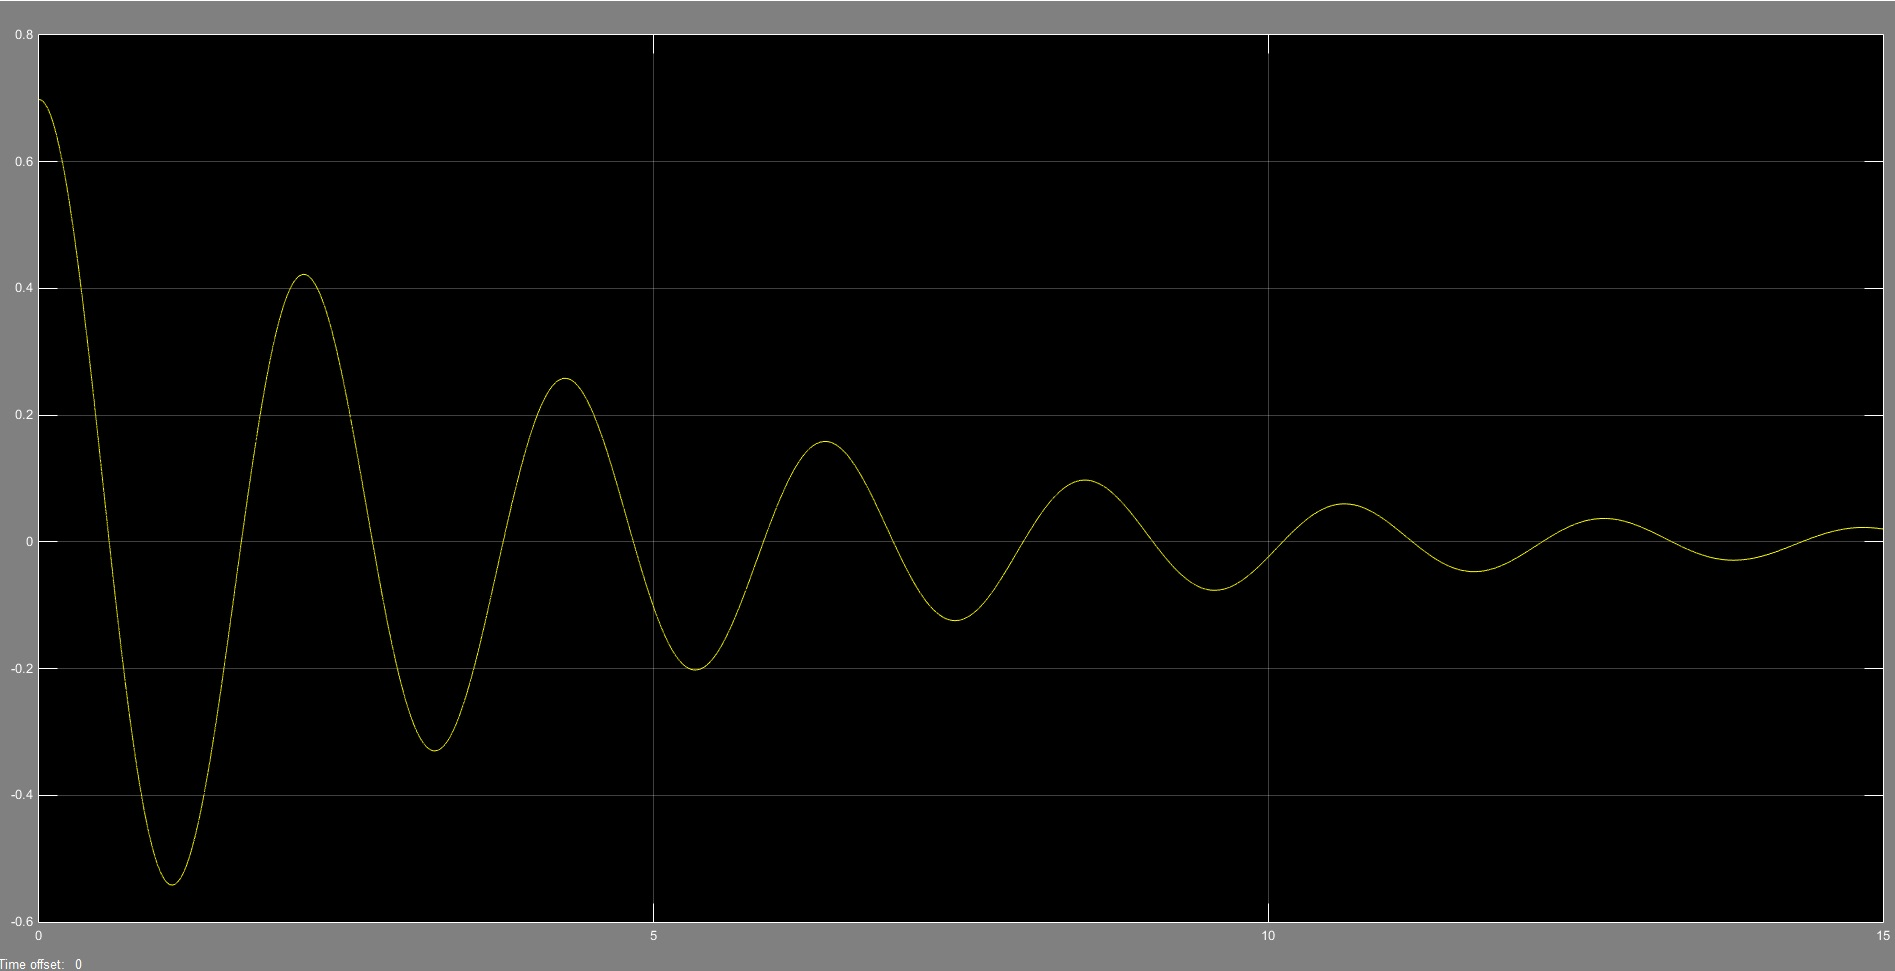
\includegraphics[width=\textwidth]{/regelung/matlab3.jpg}
%	\label{fig:matlab3}
%	\caption{Winkel $\varphi$ des Pendels über die Simulationszeit.}
%\end{figure}

%Wie erwartet, wird eine deutlich gedämpfte Schwingung des simulierten Pendels erkennbar.

\section{Simulationsblöcke}\label{sec:math-model-pmsm}

Dieses Kapitel dient zur Beschreibung der Bauteile und Komponenten, die für einen späteren Aufbau eines gesamten Regelungssystems der PMSM nötig sind.
Zunächst wird das erstellte Gesamtsystem in Abbildung \ref{fig:signalflussplan} dargestellt:

\begin{figure}[h!]
	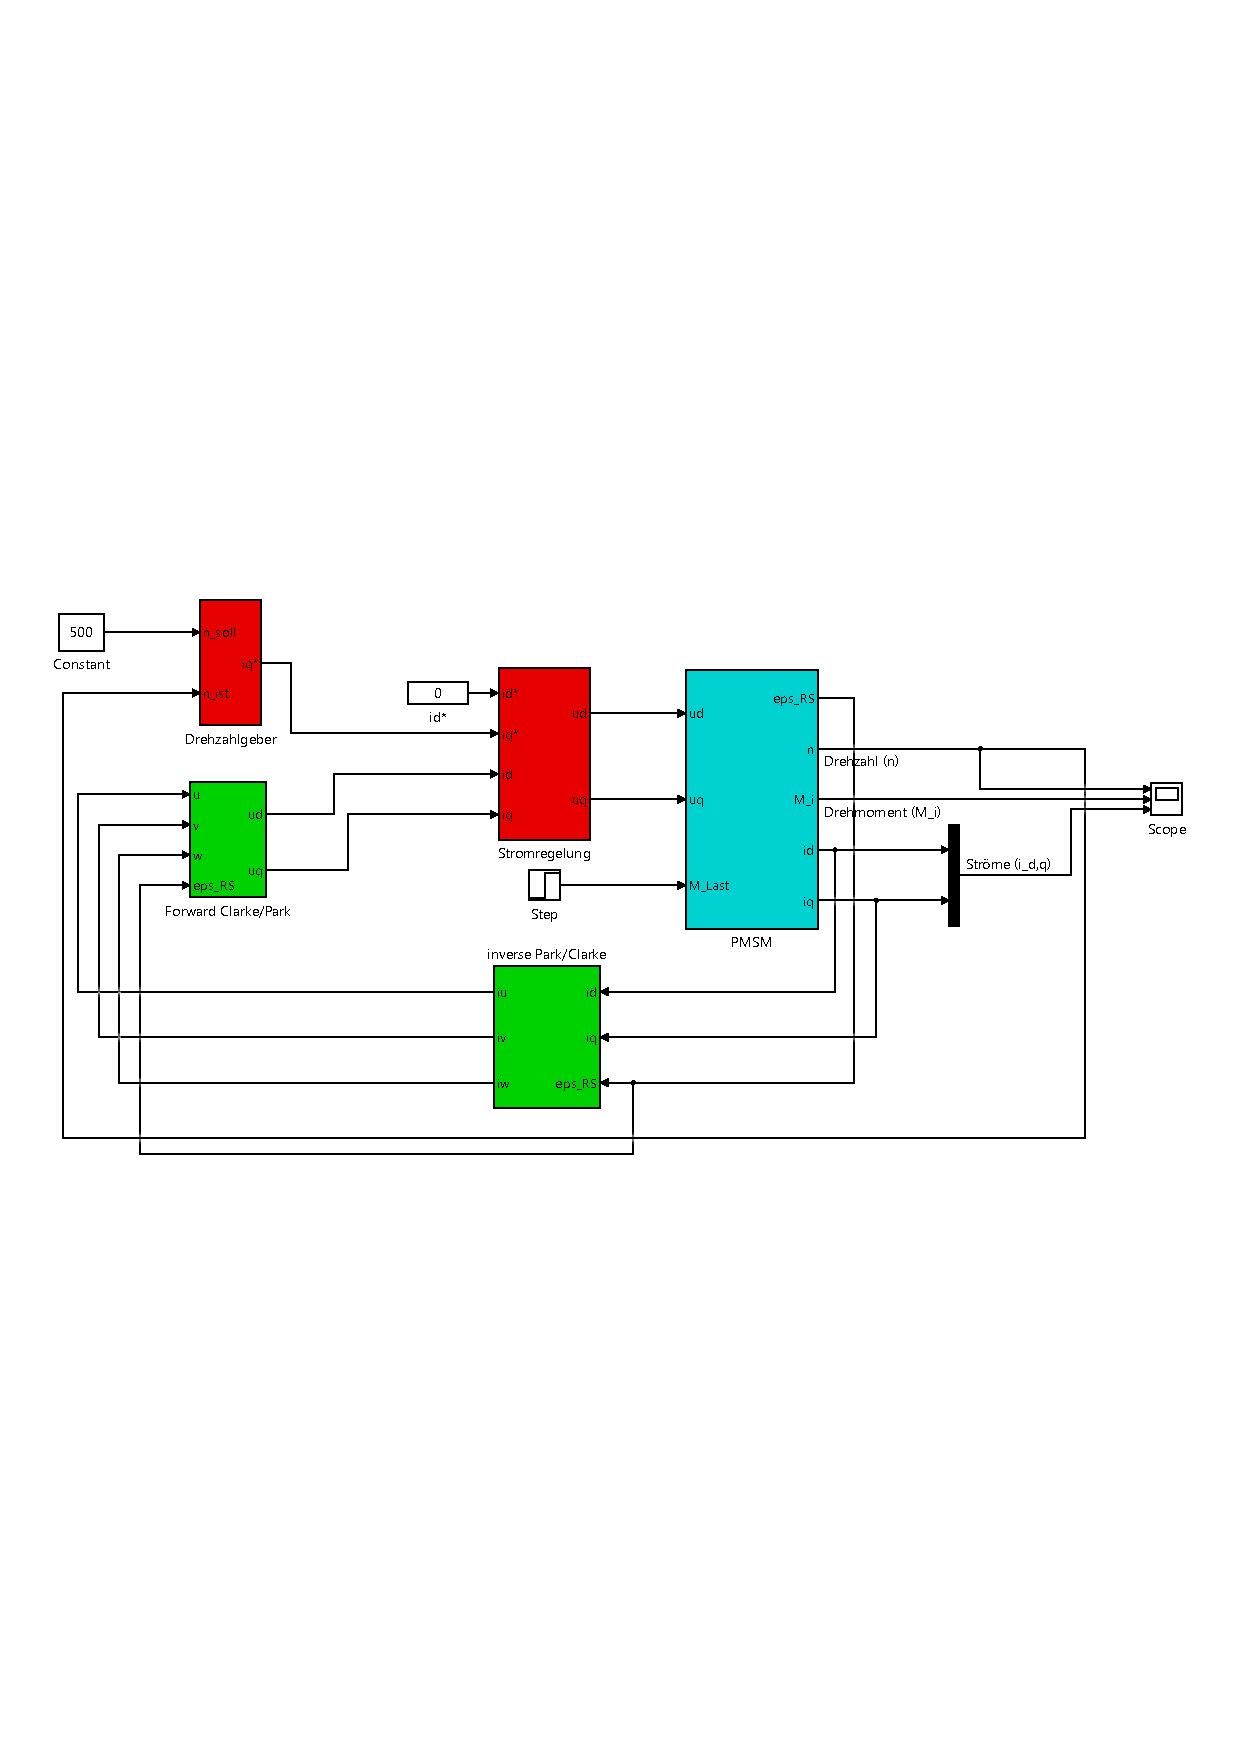
\includegraphics[width=\textwidth]{/simulink/foc-pmsm.pdf}
	\label{fig:foc-pmsm}
	\caption{Darstellung der Simulationsblöcke in Simulink.}
\end{figure}

Hier sind die Simulinkblöcke der Transformationen, das Modell der PMSM sowie Regelungskomponenten erkennbar.
Im Folgenden werden diese erläutern und deren Funktionen dargestellt.

\subsection{Transformationsblöcke}

Der Aufbau der Koordinatentransformationen leitet aus Abschnitt \ref{sec:clark} ab. 
Hierbei basiert der Block der $\alpha$-$\beta$-Transformation aus den Zusammenhängen von (\ref{clarkevektor}) und (\ref{clarkematrix}), während die Rücktransformation, die inverse $\alpha$-$\beta$-Transformation mit Hilfe von (\ref{inverseclarkevektornulleinfach}) und (\ref{inverseclarkematrixnulleinfach}) erstellt ist.
Weiterhin orientieren sich die Umsetzungen in Simulink an den Blockschaltbildern aus \ref{fig:blockbildclarkeparkkomplett} und \ref{fig:blockbildinverseclarkeparkkomplett}.

%Die folgende Abbildung \ref{fig:uvw_to_ab} zeigt den Blockaufbau der Clarke Transformation in Simulink:

%\begin{figure}[h]
%	\centering
%	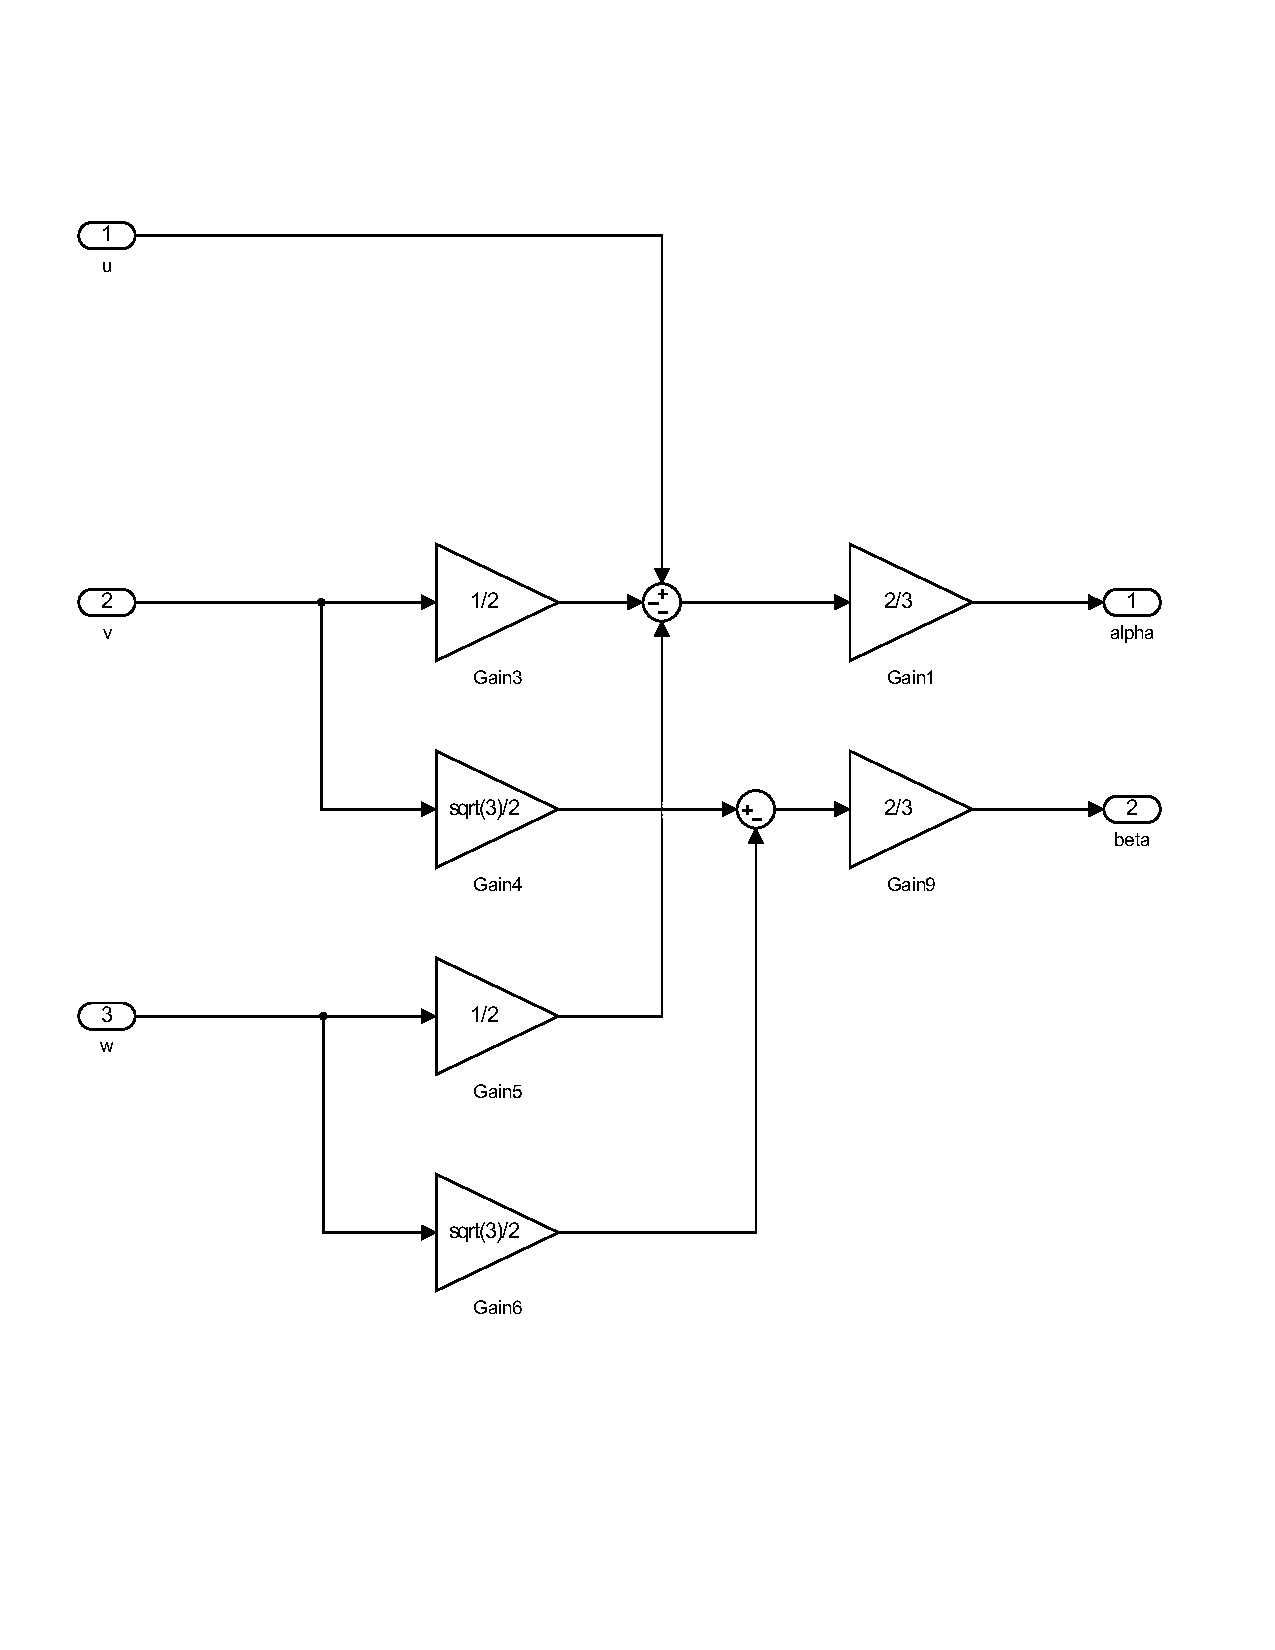
\includegraphics[width=\textwidth]{/simulink/uvw_to_ab.pdf}
%	\label{fig:uvw_to_ab}
%	\caption{Aufbau Clarke Transformation}
%\end{figure}

%In Abbildung \ref{fig:uvw_to_ab} wird der Aufbau der inversen Clarke Transformation gezeigt:

%\begin{figure}[h]
%	\centering
%	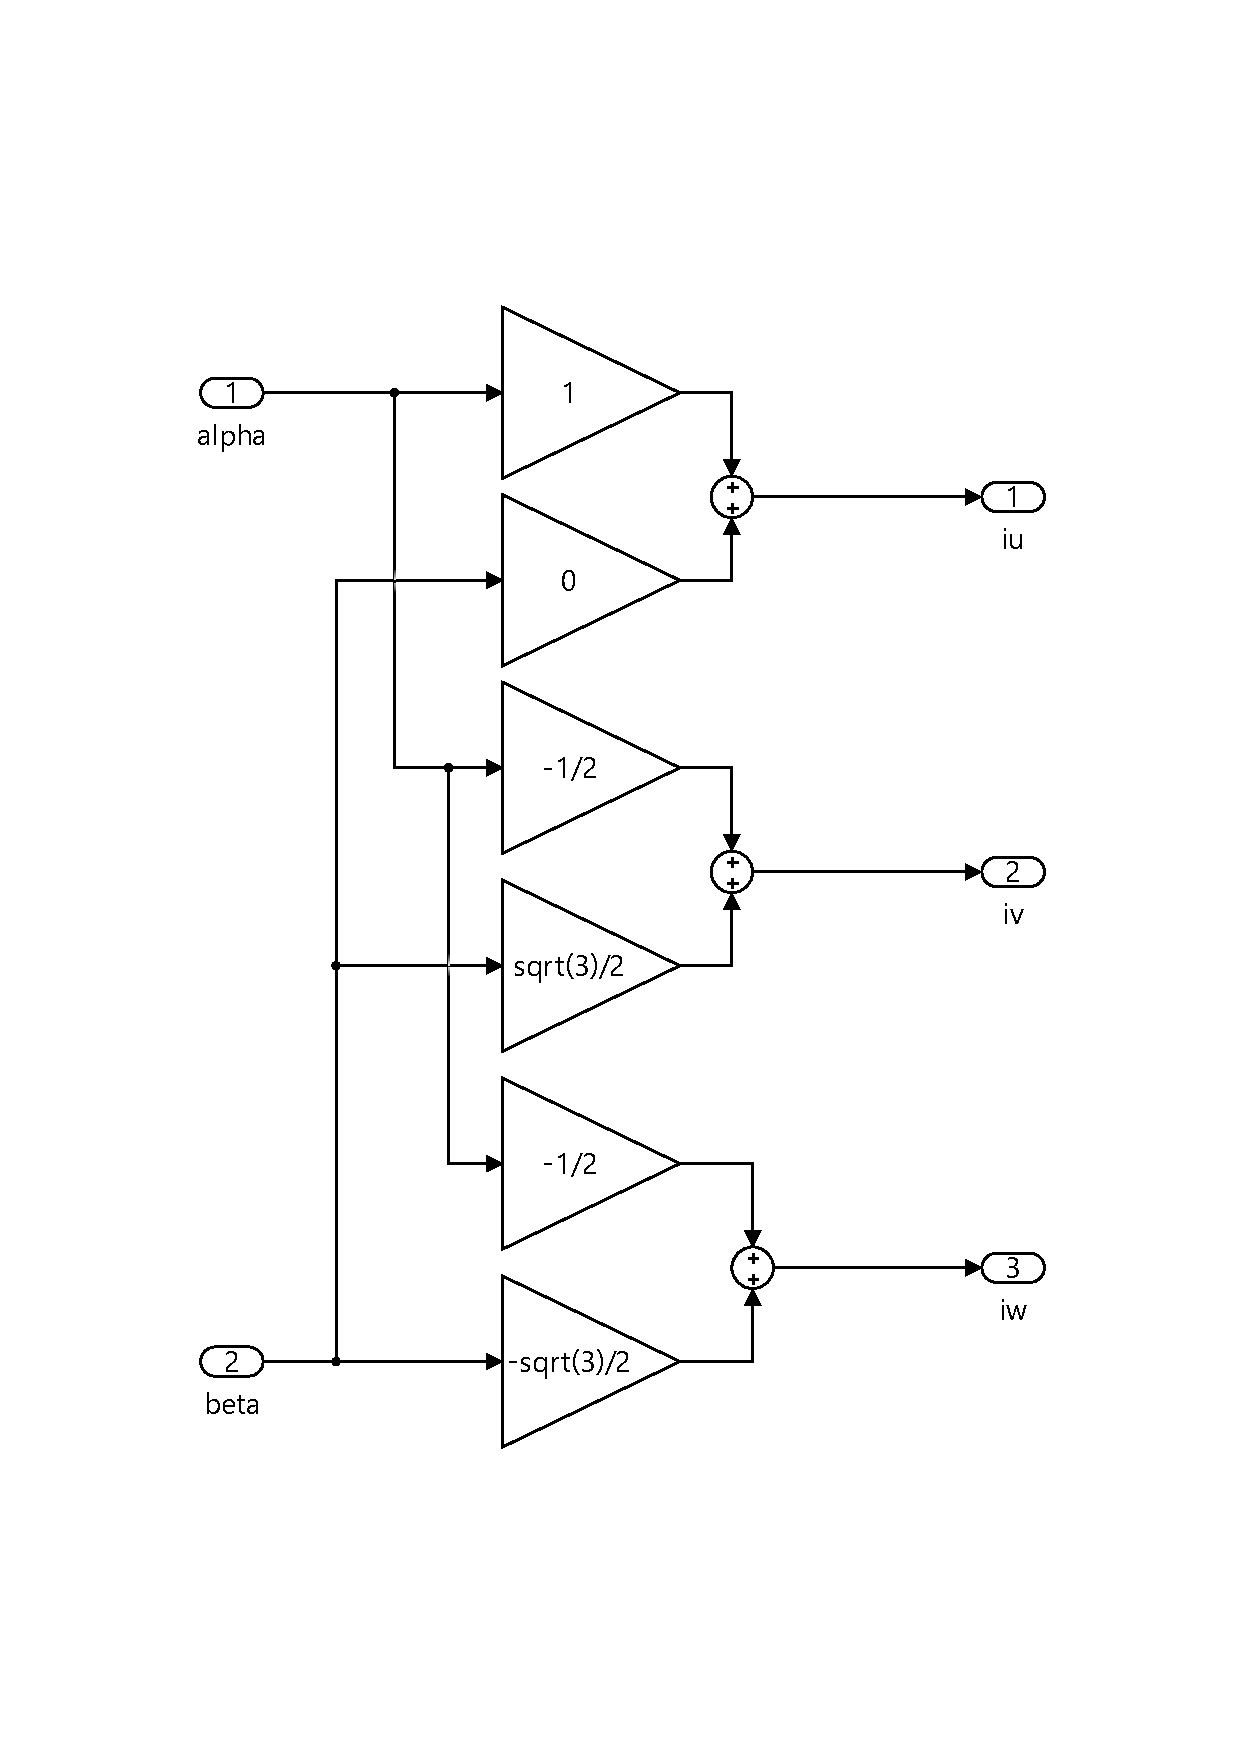
\includegraphics[width=\textwidth]{/simulink/ab_to_uvw.pdf}
%	\label{fig:ab_to_uvw}
%	\caption{Aufbau Inverse Clarke Transformation}
%\end{figure}

Um die Koordinatentransformation zu vervollständigen ist die d-q-, oder Park Transformation, von entscheidender Bedeutung.
Der Block für die d-q-Transformation setzt wird mit dem Zusammenhang \ref{parkvektor} und der Matrix \ref{parkmatrix} erstellt. 
Die inverse d-q-Transformation ist mit Hilfe der Matritzen \ref{parkvektorinvers} sowie \ref{parkmatrixinvers} aufgebaut.

%Die nachstehende Grafik \ref{fig:ab_to_dq} stellt die Park Transformation in Simulink dar:

%\begin{figure}[h]
%	\centering
%	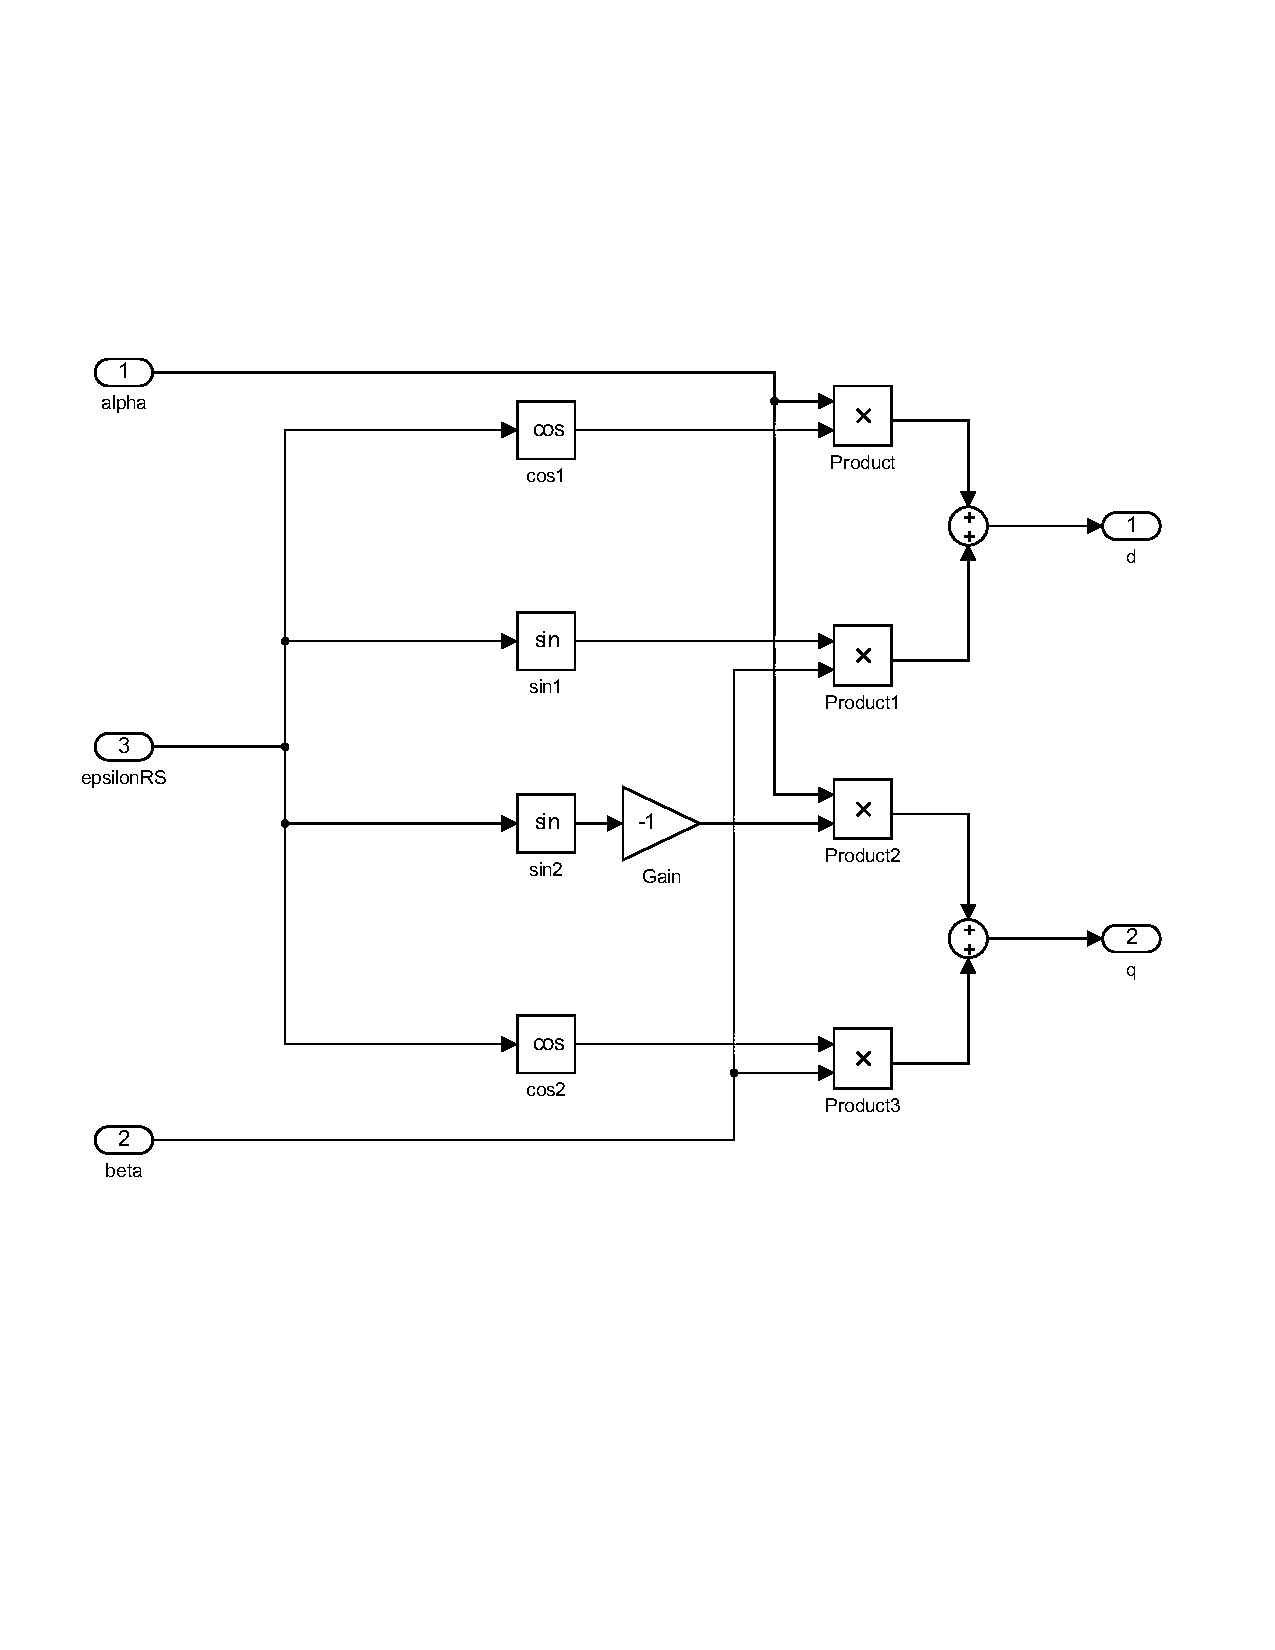
\includegraphics[width=\textwidth]{/simulink/ab_to_dq.pdf}
%	\label{fig:ab_to_dq}
%	\caption{Aufbau Park Transformation}
%\end{figure}

%In Abbildung \ref{fig:dq_to_ab} ist der Aufbau der inversen Park Transformation dargestellt:

%\begin{figure}[h]
%	\centering
%	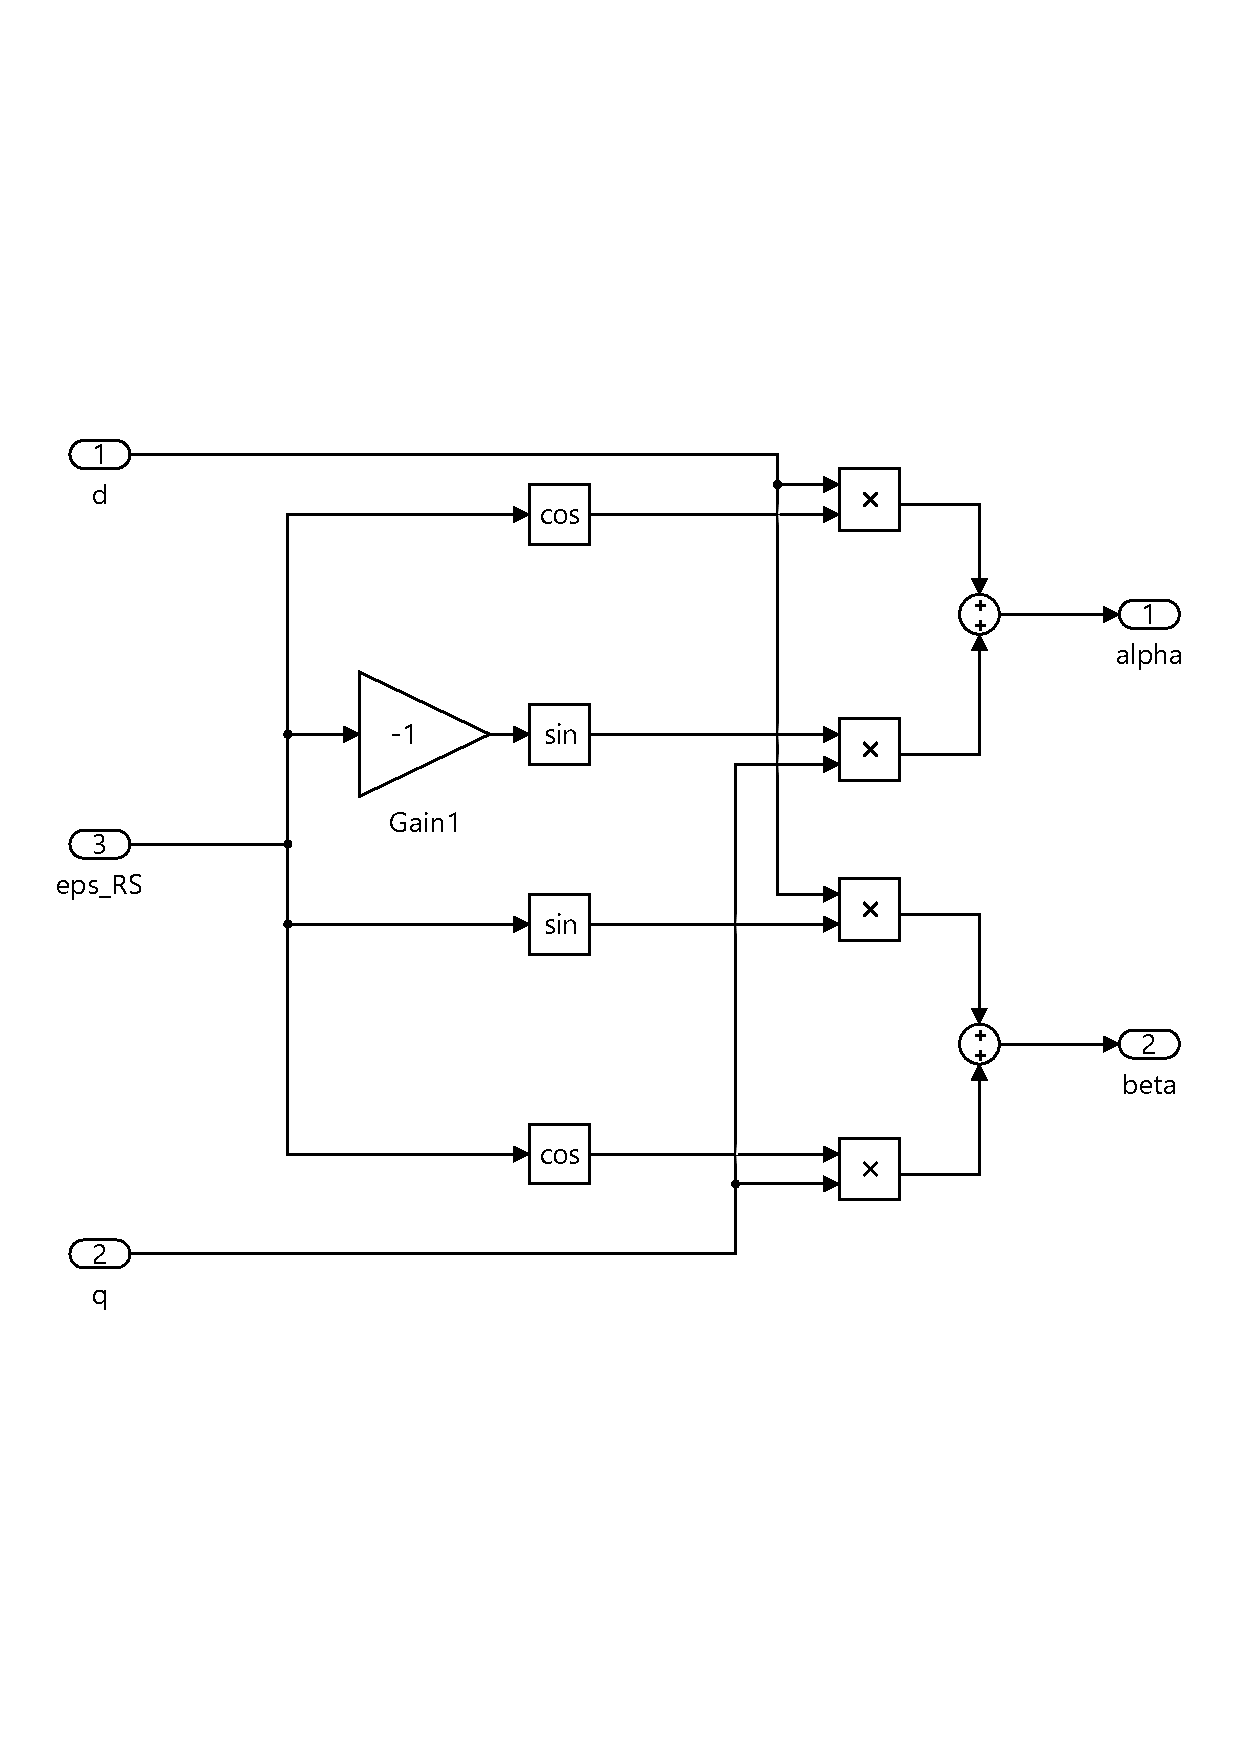
\includegraphics[width=\textwidth]{/simulink/dq_to_ab.pdf}
%	\label{fig:dq_to_ab}
%	\caption{Aufbau Inverse Park Transformation}
%\end{figure}

An dieser Stelle ist es aus übersichtlichkeitsgründen sinnvoll, die Transformationsblöcke als Subsystem zusammenzufassen.
Es ergibt sich für die Clarke-Park Transformation somit ein Block mit drei Eingängen für die drei Wechselgrößen und einem Eingange für $\varepsilon_\i{RS}$, sowie zwei Ausgängen für d- und q-Komponente.
Ebendieses wird auch für die Rücktransformation gemacht. 
Hier ergibt sich ein Subsystem mit drei Eingängen. 
Zwei für d- und q-Größe sowie ebenfalls ein Eingang für $\varepsilon_\i{RS}$.
Es ergeben sich drei Ausgänge für das rückgeführte Dreiphasensystem.

\newpage
\begin{figure}[h]
	\centering
	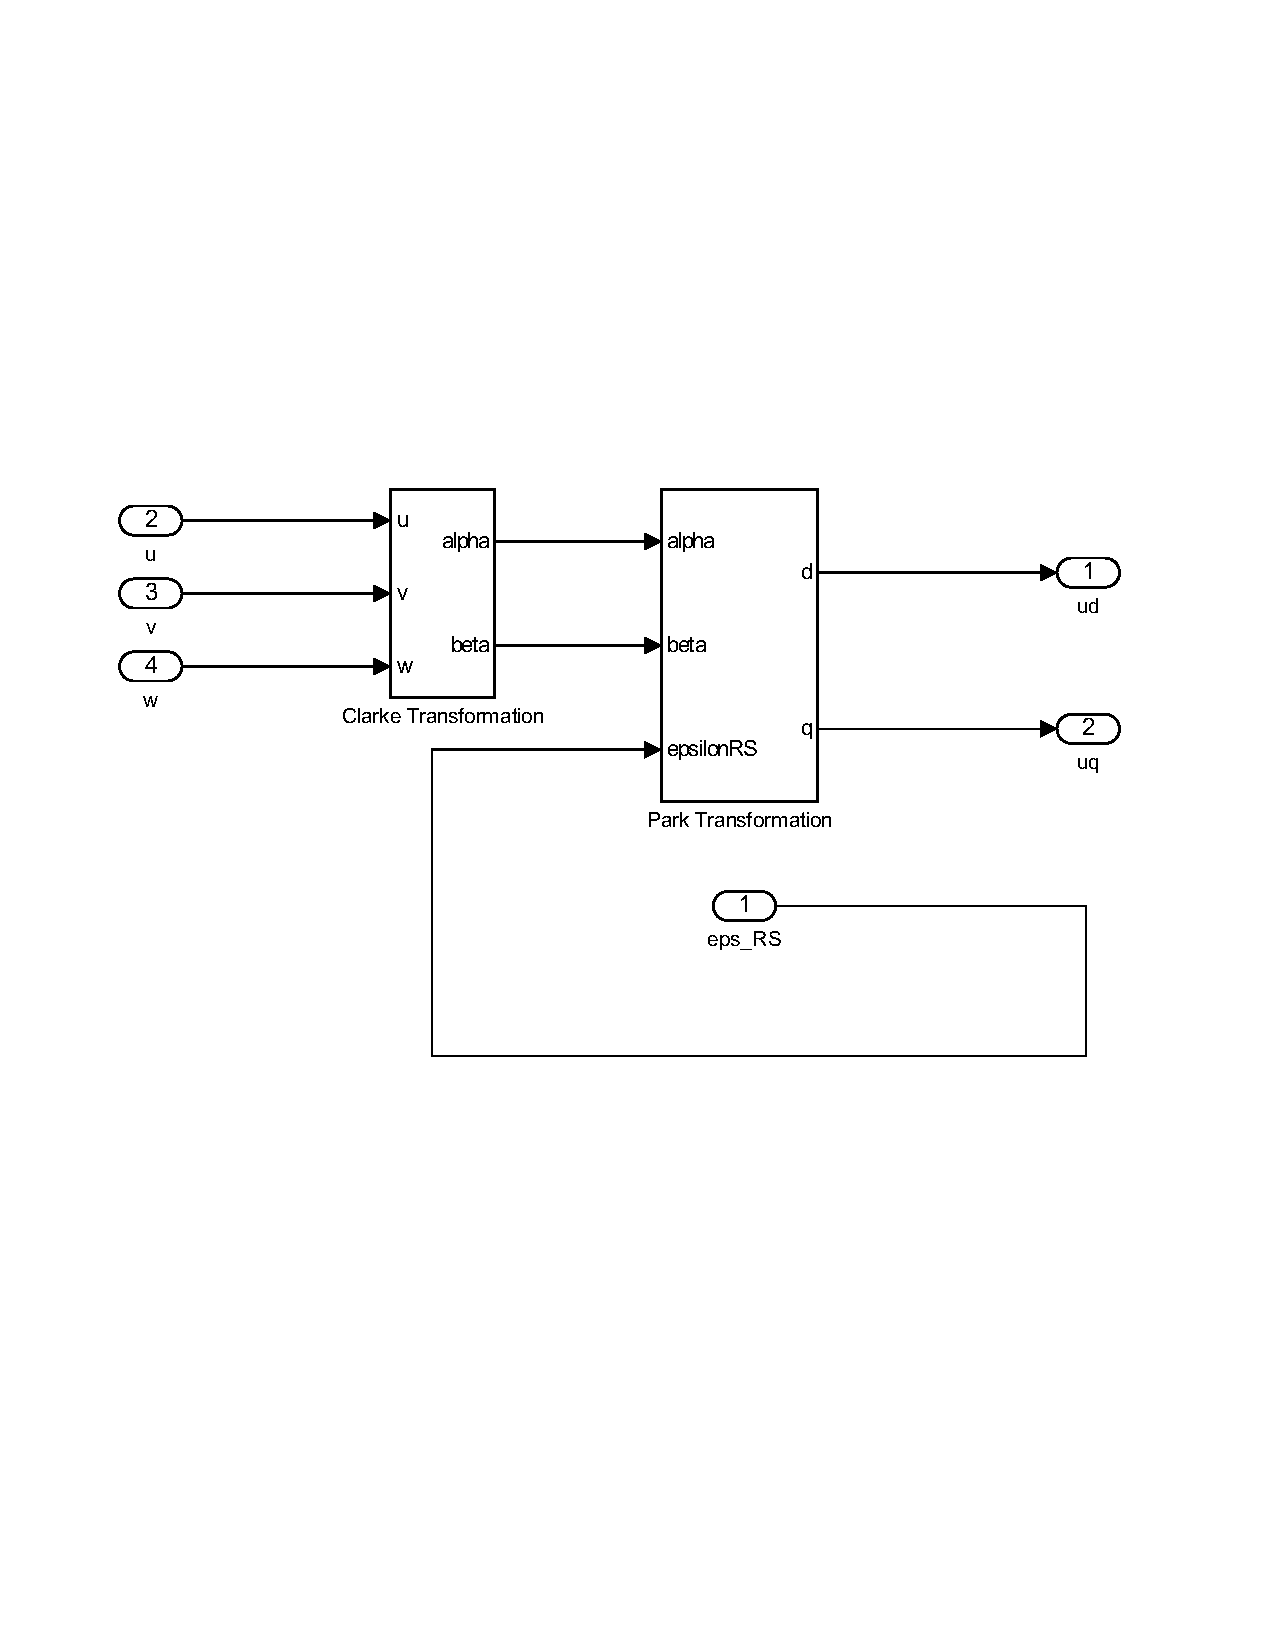
\includegraphics[width=\textwidth]{/simulink/uvw_to_dq.pdf}
	\label{fig:uvw_to_dq}
	\caption{Aufbau Clarke-Park Transformation}
\end{figure}

\begin{figure}[h]
	\centering
	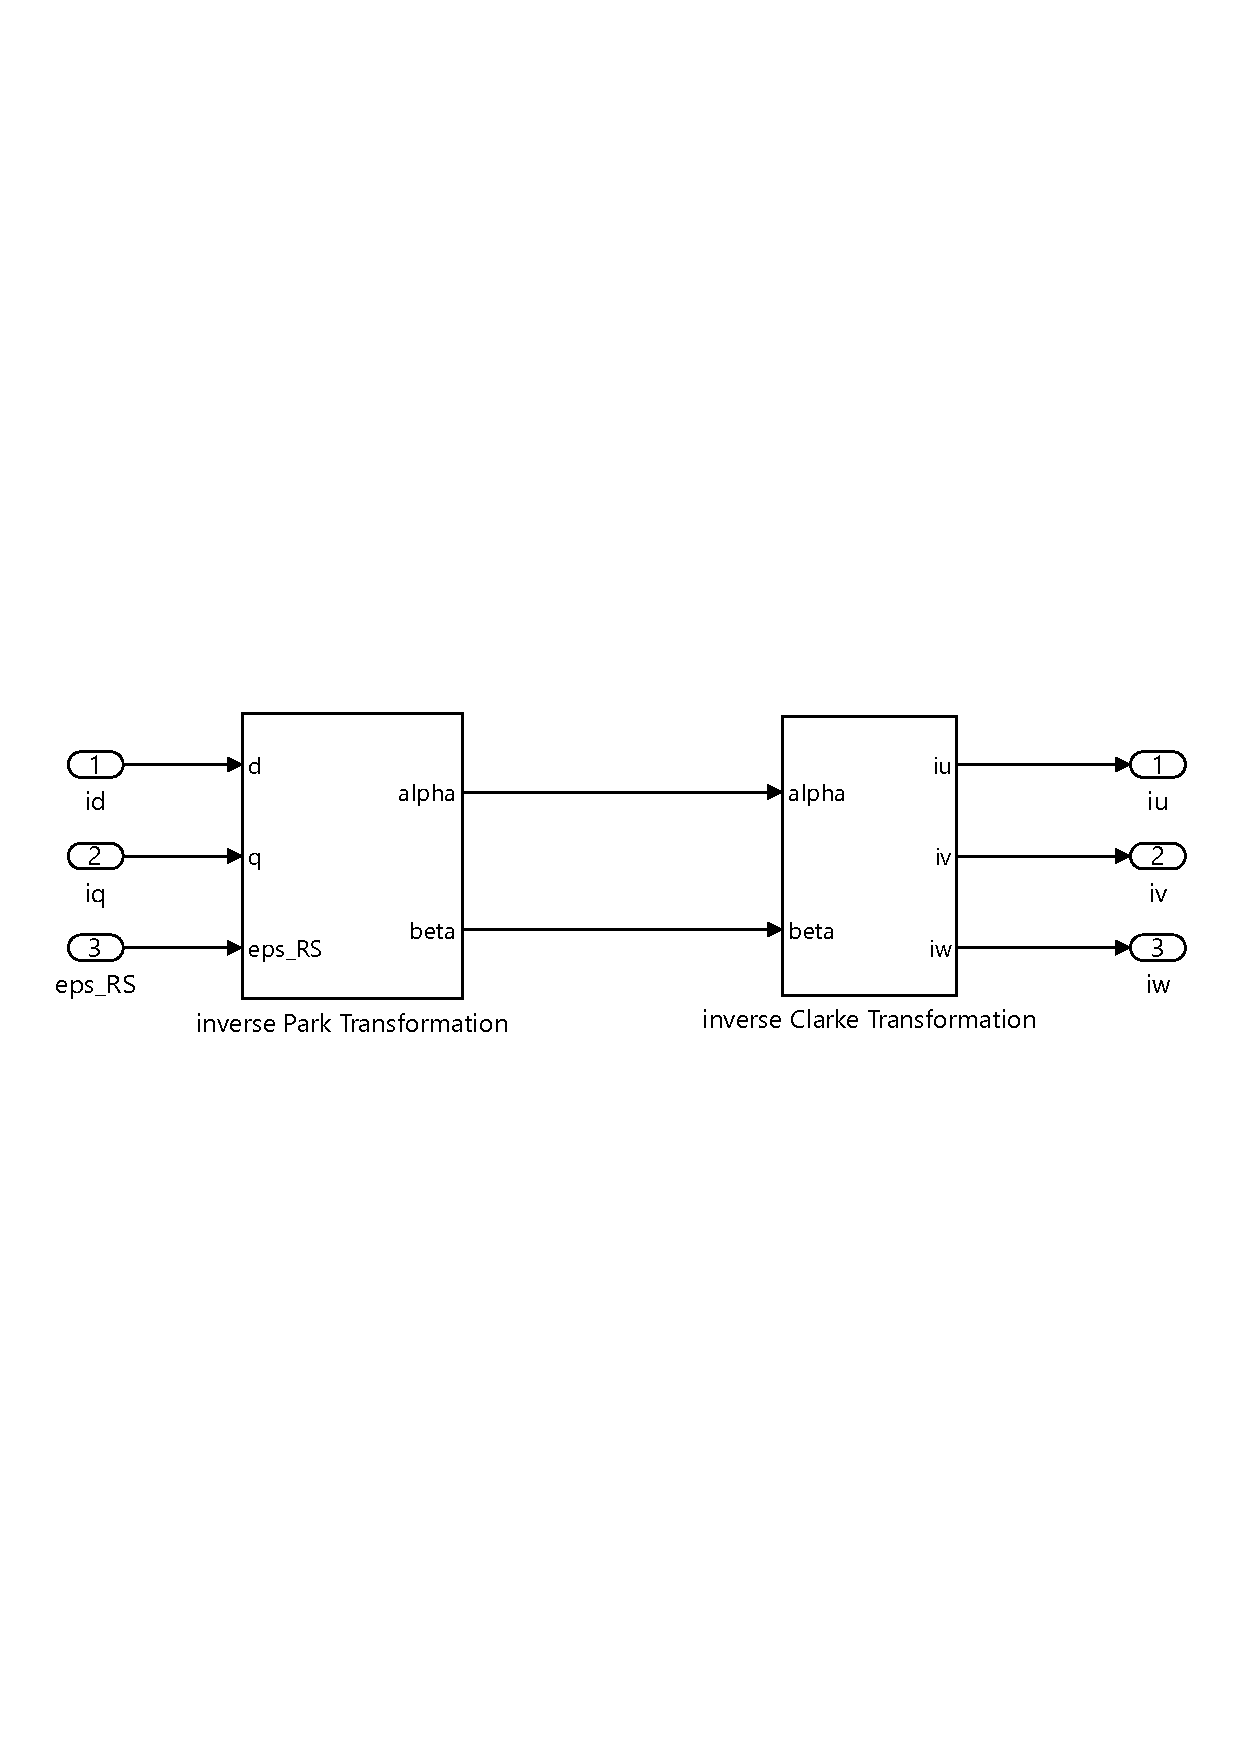
\includegraphics[width=\textwidth]{/simulink/dq_to_uvw.pdf}
	\label{fig:dq_to_uvw}
	\caption{Aufbau inverse Clarke-Park Transformation}
\end{figure}
\newpage

\subsection{Modellierung einer PMSM}

Als Grundlage für die Betrachtung der PMSM gilt der Abschnitt \ref{sec:synchron-dq}.
Die grundlegenden Gleichung dazu sind (\ref{eqn:ud-lin-gleichung}), (\ref{eqn:uq-lin-gleichung}) und (\ref{eqn:mi-lin-gleichung}).
Aus den Gleichungen ergibt sich im Simulink das Modell.
Das Modell wird in zwei Systeme unterteilt:

\begin{itemize}
	\item Mechanical system
	\item Electrical system
\end{itemize}

\begin{figure}[h!]
	\centering
	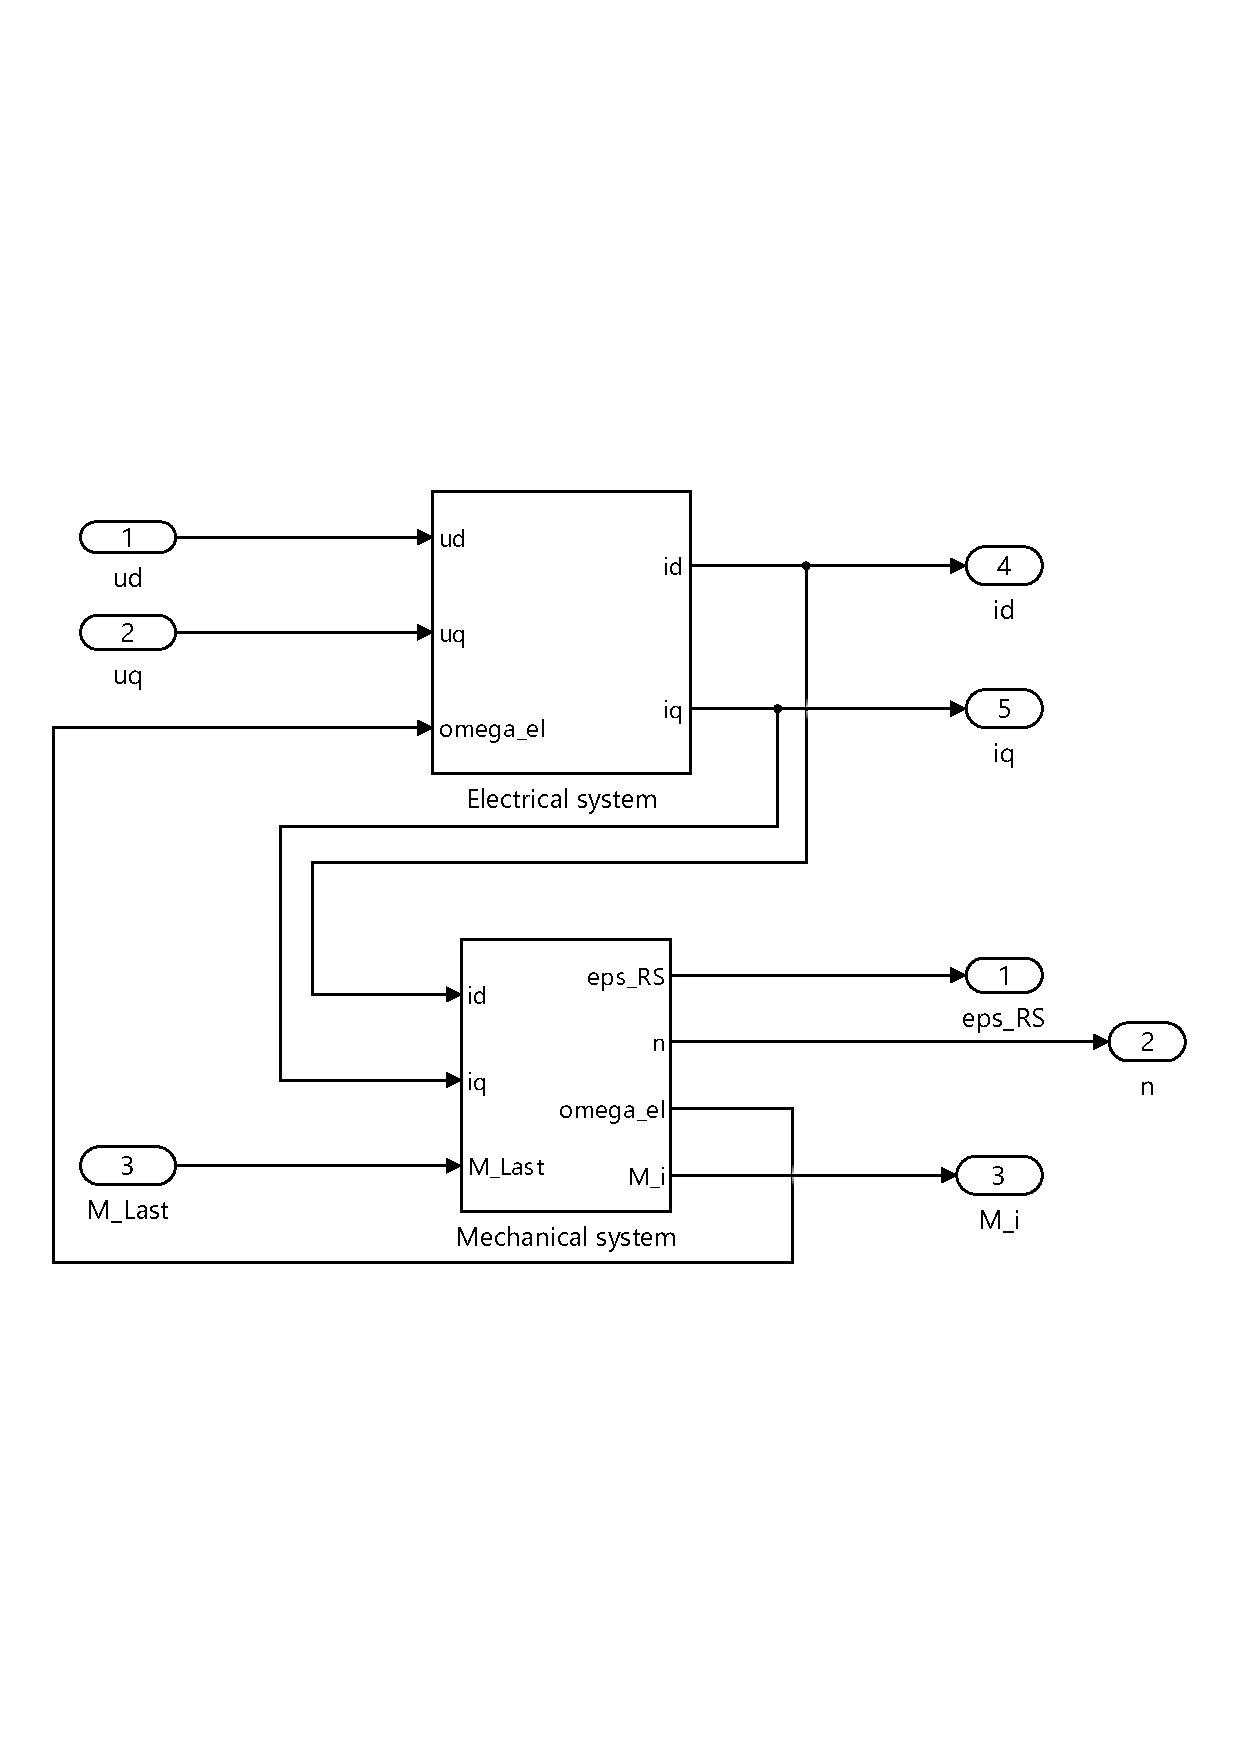
\includegraphics[scale=0.7]{/simulink/pmsm.pdf}
	\label{fig:pmsm}
	\caption{Aufbau des Subsystems: PMSM, mit der Unterteilung in: Electrical system und Mechanical system.}
\end{figure}

Bei dem \enquote{Mechanical system} wird die Differentialgleichung der elektrischen Winkelgeschwindigkeit beschrieben s.~h.~Gl.~(\ref{eqn:mi-lin-gleichung}).
Das \enquote{Electrical system} beschreibt hingegen die Differentialgleichungen der Ströme und somit die elektrischen Parameter einer PMSM.
Die Überführung der Maschinengleichungen erfolgt dabei dem gleichen Prinzip wie in Abschnitt \ref{cha:regelungpmsm}.
Zunächst wird auf das \enquote{Electrical system} eingegangen, welches in Abbildung \ref{fig:electrical-system} dargestellt ist.
Die dabei modellierten Differentialgleichungen~(\ref{eqn:id_dt}) und (\ref{eqn:iq_dt}) werden entsprechend umgesetzt, dabei entsteht das Modell auf Basis eines vereinfachten Modells (s.~h.~Abschnitt~\ref{sec:synchron-dq}~--~Linearisierte Gleichungen (Spannungsgleichungen im rotorfesten System)).
Aus der Bestimmungsgleichung~(\ref{eqn:mi-lin-gleichung}) folgt die elektrische Winkelgeschwindigkeit $\omega_\x{el}$ (s.~h.~Gl.~(\ref{eqn:dw_dt})).

\subsection{Regelungtechnische Blöcke}

Wie in der Abbildung \ref{fig:foc-pmsm} erkennbar ist, sind reglungstechnische Elemente enthalten.
Zum einen ein Drehzahlgeber (s.~h.~Abbildung~\ref{fig:drehzahl}) und zum anderen die Stromregelung (s.~h.~Abbildung~\ref{fig:stromregelung}).
Wie schon im Abschnitt~\ref{sec:foc} erörtert, regelt die Stromregelung den $i_\x{q}$-Strom~--~damit wird das benötigte Drehmoment realisiert.
Der Drehzahlgeber führt dem System die eingestellte Drehzahl zur Verfügung, so dass die Kombination aus Drehzahlgeber und Stromregelung an einem gemeinsamen Strang ziehen.
Die Stromregelung wird durch zwei einfache PI-Regeler realisiert.
Auch der Drehzahlgeber wird lediglich durch einen PI-Regler realisiert.
Komplexere Regler werden für die feldorientierte Regelung nicht benötigt \autocites{Perassi2006}{kellner2012}.

\begin{figure}[h]
	\centering
	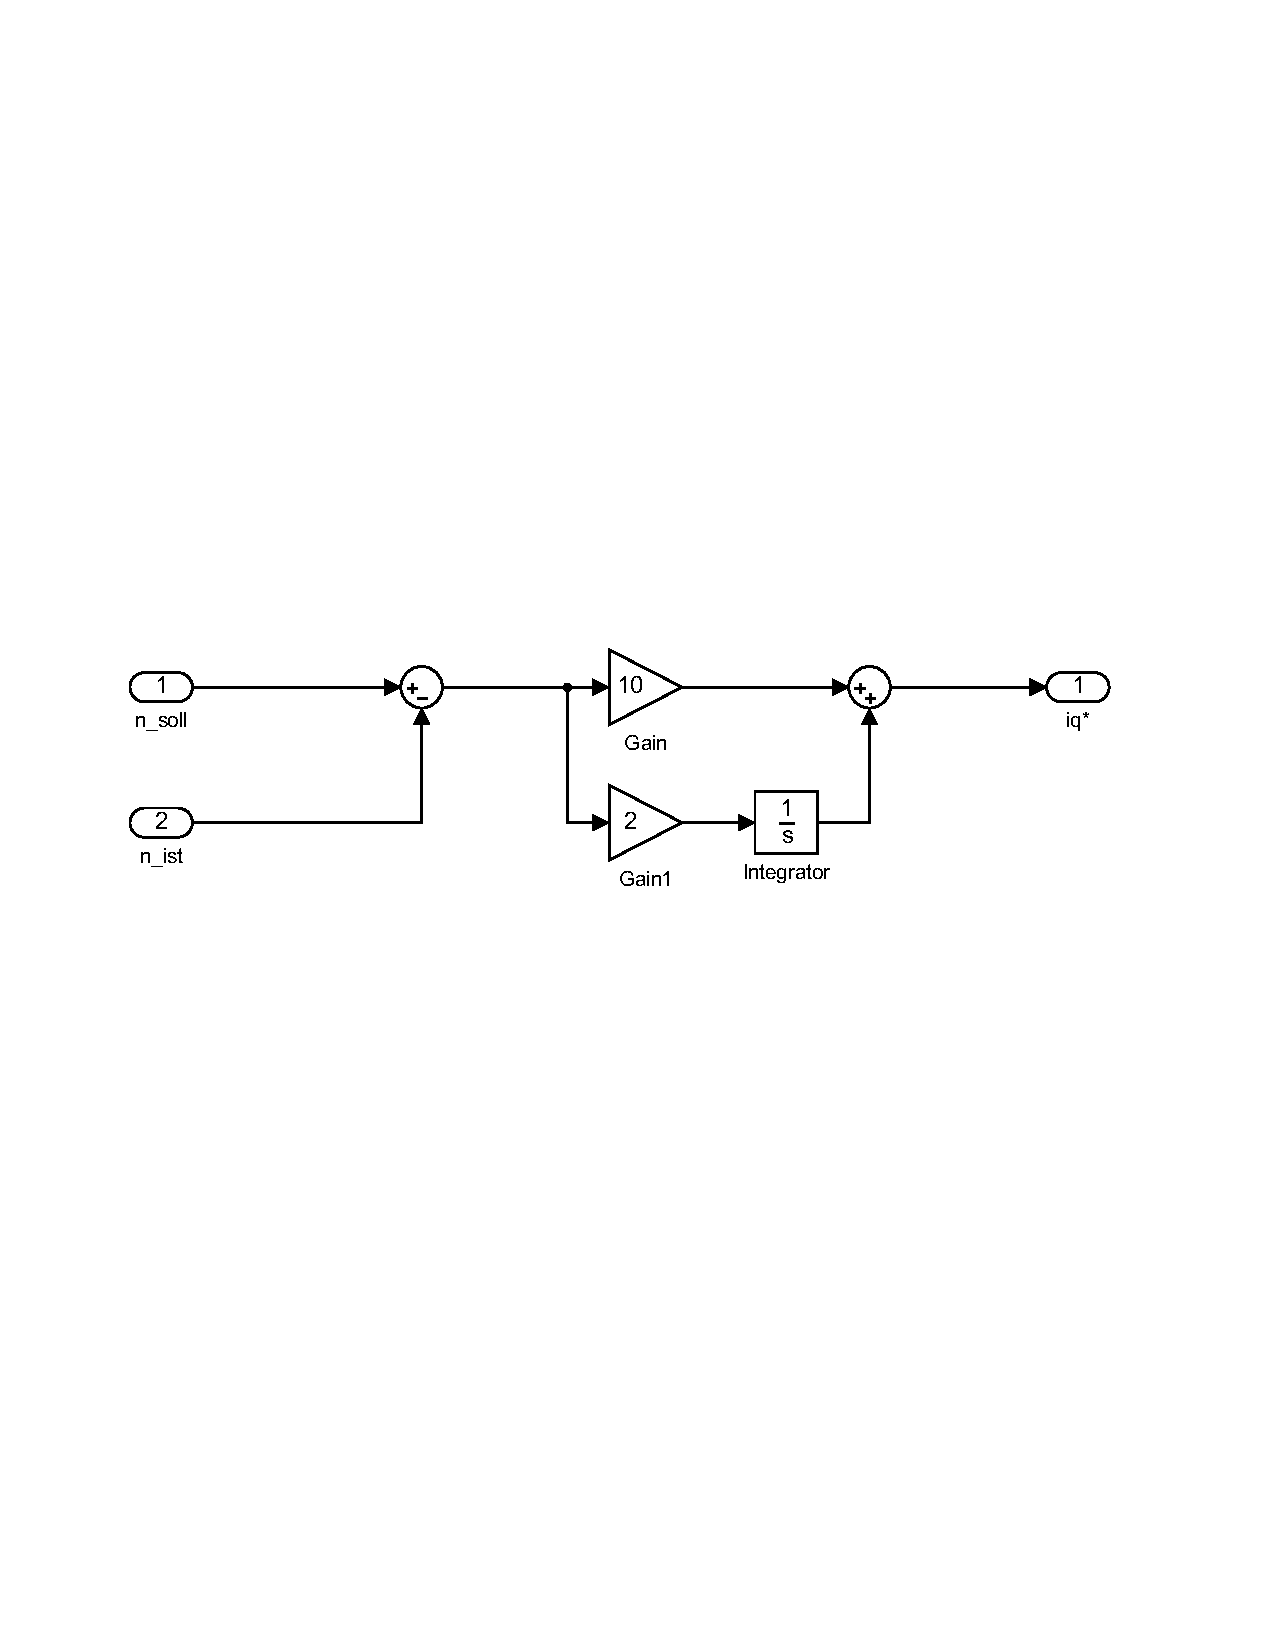
\includegraphics[width=\textwidth]{/simulink/drehzahl.pdf}
	\label{fig:drehzahl}
	\caption{Aufbau der Drehzahlregelung.}
\end{figure}

\begin{figure}[h]
	\centering
	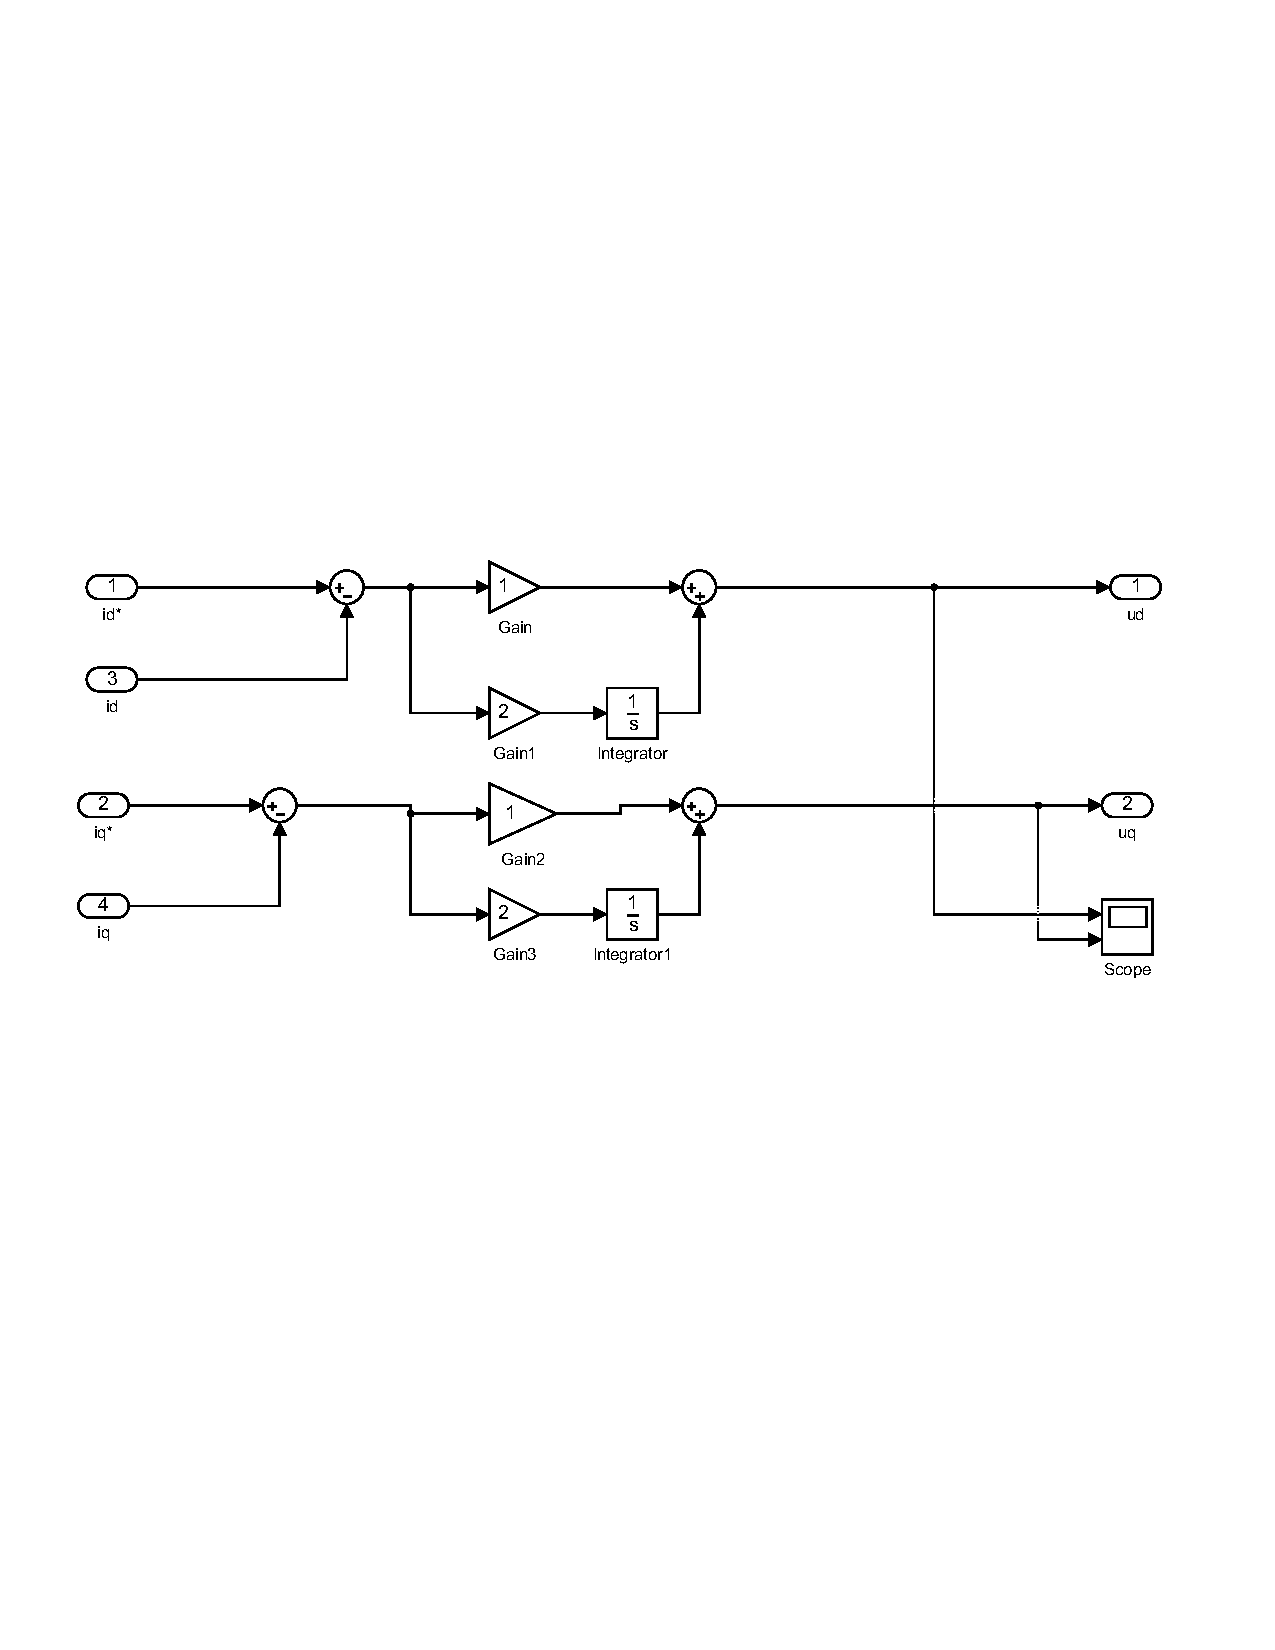
\includegraphics[width=\textwidth]{/simulink/stromregelung.pdf}
	\label{fig:stromregelung}
	\caption{Aufbau der Stromregelung.}
\end{figure}

Der PI-Block aus der \enquote{Simulink $\rightarrow$ Modeling $\rightarrow$ Block Libraries $\rightarrow$ Continous} Bibliothek ist standardmäßig als \enquote{Continuos-time} Block konfiguriert.
Hinter dem Block stecken ähnlich wie in Abbildung \ref{fig:foc-dc-ac} veranschaulicht eine einfache mathematische Gleichung.
Zudem sei gesagt, dass eine Parallele Regelstruktur angenommen wird.

\begin{align}
	P + I\cdot\frac{1}{s}
\end{align}

Dabei steht $P$ für die Verstärkung des Reglers und $I$ für die Verstärkung des Integralen Anteils.

\begin{quote}
	\enquote{[\ldots] Specify the proportional gain P. [\ldots] Specify the integral gain I. [\ldots] (Mathworks Help -- PID Controller, Discrete PID Controller. In: Simulink $\rightarrow$ Modeling $\rightarrow$ Block Libraries $\rightarrow$ Continous)}
\end{quote}

%%% Local Variables: 
%%% mode: latex
%%% TeX-master: "main"
%%% TeX-open-quote: "\\enquote{"
%%% TeX-close-quote: "}"
%%% LaTeX-csquotes-open-quote: "\\enquote{"
%%% LaTeX-csquotes-close-quote: "}"
%%% End: 

% -*- coding: utf-8 -*-
% !TEX encoding = UTF-8 Unicode
% !TEX root =  main.tex

\chapter{Zusammenfassung}
\label{cha:zusammenfassung}

Die Zielsetzung des Projektes ist die vollständige Implementierung einer Vektorregelung für Synchronmaschinen in \product{Matlab/Simulink} unter Verwendung der Bibliotheken für Texas Instruments DSPs.
Zu den Aufgabenstellungen die erfüllt wurden, gehört eine ausführliche Literaturrecherche zum Maschinenmodell einer anisotropen Synchronmaschine und die Implementierung des mathematischen Modells in \product{Simulink}.
Im Rahmen des Projektes wurde eine ausführliche und übersichtliche Dokumentation zu den oben aufgeführten Aufgaben erstellt.
Beiliegend eine CD mit dem Maschinenmodell und den benutzten \product{Simulink} Bausteinen.
%Der Vergleich mit der Texas Instrument Bibliothek gestaltete sich als schwierig und sehr aufwändig.
%Die Lauffähigkeit der Modelle stellte sich als nicht stabil heraus, da Änderungen an den Parametern zu unerwünschten Effekten führte.
Die Lauffähigkeit der Modelle ist nicht gewährleistet, weil zum einen die synchrone Drehzahl bei der Simulation mit starren Netz nicht erreicht wurde (s.~h.~Abschnitt~\ref{sec:sim-starr-netz}) und zum anderen führten Parameter Änderungen zu unerwünschten Nebeneffekten (z.\~B.\ die Drehzahl ist während des Einschwingvorganges negativ geworden).
Durch das vernachlässigen der Sättigung der Blechpackete bei den Modellen, werden die Ströme während des Einschwingvorganges sehr hoch (s.~h.~Abbildung~\ref{fig:drehmoment}).
Die Clarke/Park-Transformation ist bei dem Modell mit starren Netz nicht wie erwartet gleichförmig gewesen (s.~h.~Abbildung~\ref{fig:n-netz}).
Bestehende Modelle der TI-Bibliothek sind nicht zum Vergleich geeignet gewesen, da diese mit einer Raumzeigermodulation modelliert sind und somit nicht zum Vergleich mit dem Starren Netz möglich waren.
Außerdem waren viele Modelle mit der Bibliothek von Simscape ausgestattet, so dass ein Vergleich nicht sinnvoll war.
Das Modell mit der PWM funktioniert entspricht den Anforderungen an Funktionalität.

Für zukünftige Arbeiten in diesem Bereich empfiehlt sich eine ausführliche Literaturrecherche für die TI-Bausteine und die Implementierung von \enquote{Saturation-Blocks}.
Die Sättigung der Blechpackete scheint von größerer Bedeutung zu sein, als angenommen.
Zusätzlich ist es notwendig die Parameter der Regelung besser einzustellen, da diese einen sehr großen Einfluss auf die dargestellten Ergebnisse im Kapitel~\ref{chap:ergebnisse-foc} haben.
Die Problematik mit der Clarke/Park-Transformation stellt sich als ungelöst dar und muss entsprechend korrigiert werden, damit das Modell funktionsfähig wird.
Zusätzlich bietet es sich an andere Simulationsverfahren zu verwenden, wie z.\ B.\ Verfahren mit variabler Schrittweite.



%%% Local Variables: 
%%% mode: latex
%%% TeX-master: "main"
%%% TeX-open-quote: "\\enquote{"
%%% TeX-close-quote: "}"
%%% LaTeX-csquotes-open-quote: "\\enquote{"
%%% LaTeX-csquotes-close-quote: "}"
%%% End: 

\listoffigures
% ----------------------------------------------------------------------------------------------------------
% Literatur
% ----------------------------------------------------------------------------------------------------------
\cleardoublepage
\nocite{*}
\printbibliography
% ----------------------------------------------------------------------------------------------------------
% Anhang
% ----------------------------------------------------------------------------------------------------------
\begin{appendix}
\chapter{Simulationsblöcke}
\section{Elektrische Komponenten}
\begin{figure}[htb]
	\centering
	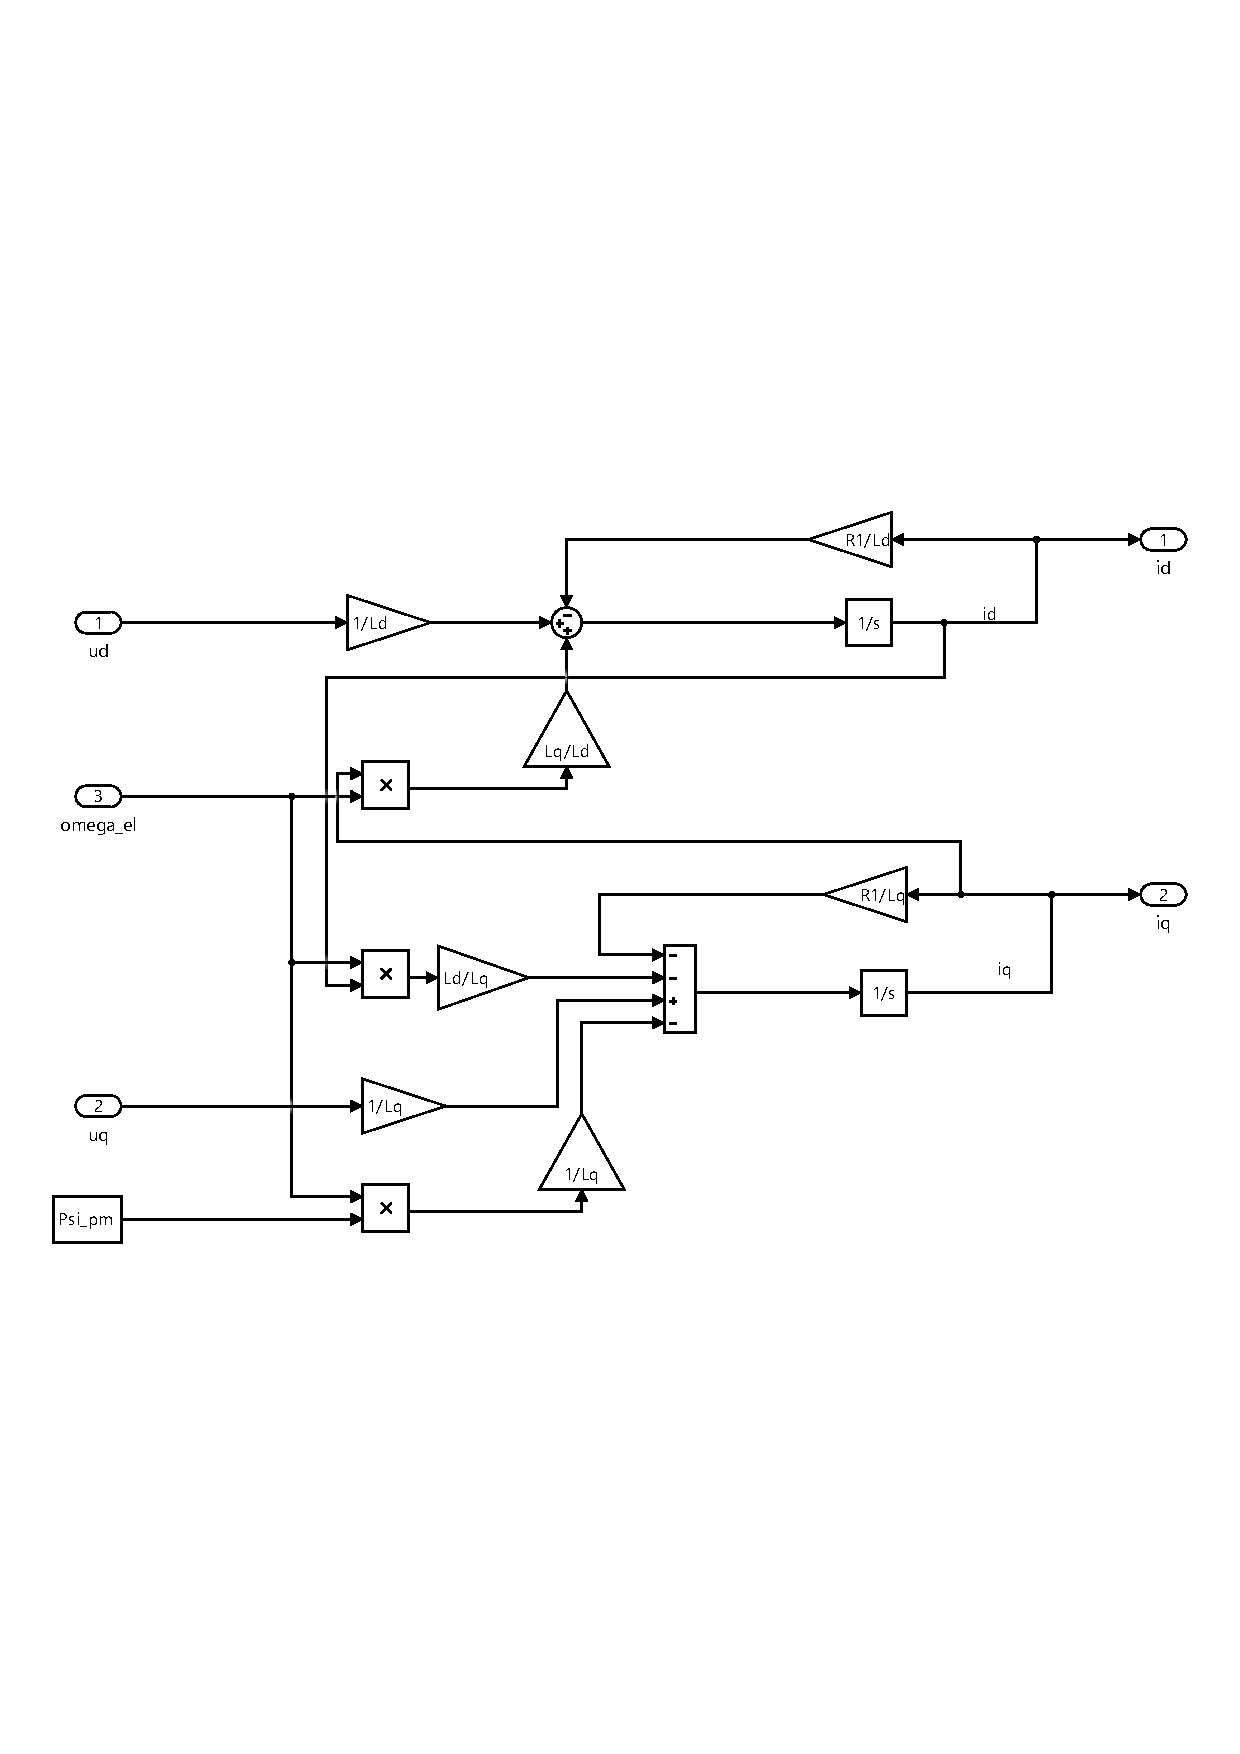
\includegraphics[width=\textwidth]{/simulink/electrical-system.pdf}
	\label{fig:electrical-system}
	\caption{Aufbau des elektrischen Subsystemsystems.}
\end{figure}

\begin{figure}[htb]
\centering
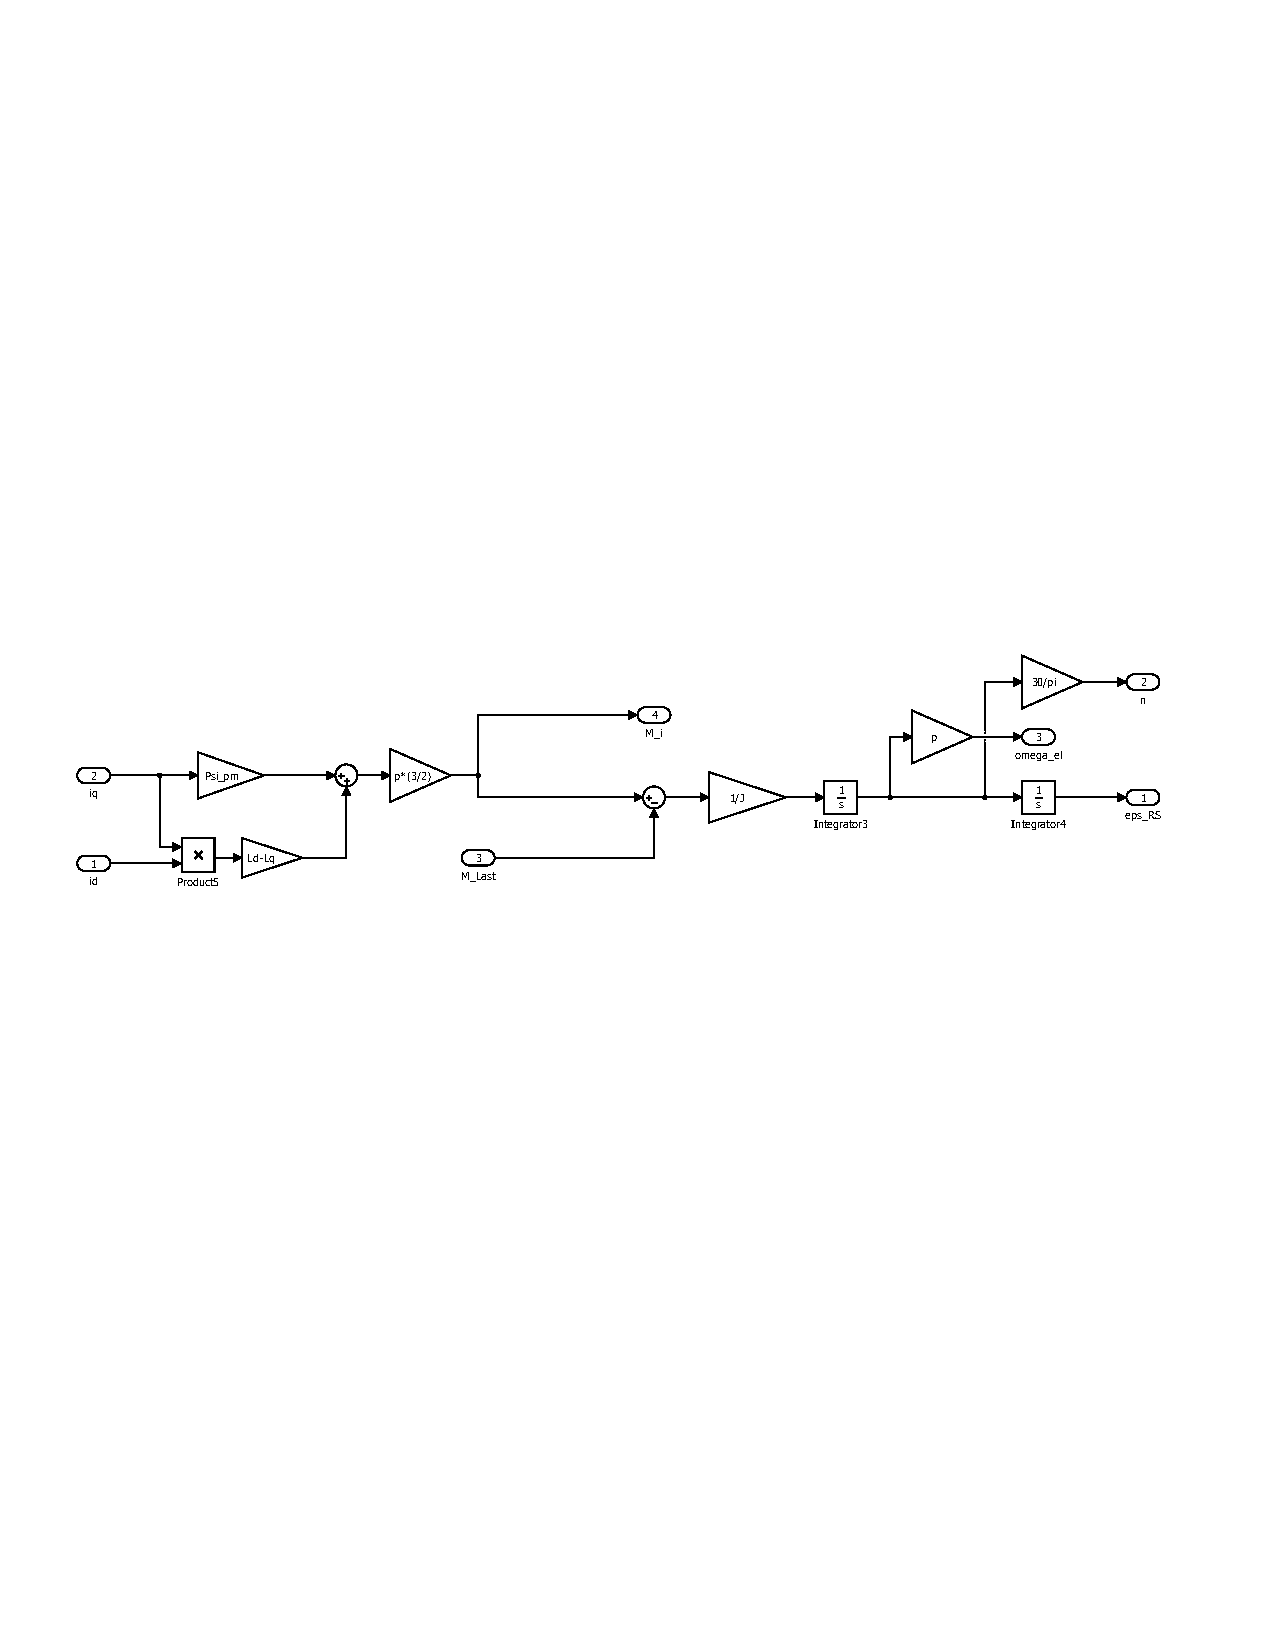
\includegraphics[width=\textwidth]{/simulink/mechanical-system.pdf}
\label{fig:mechanical-system}
\caption{Aufbau des mechanischen Subsystems.}
\end{figure}
\newpage
\section{Reglungstechnische Komponenten}
\begin{figure}[h]
	\centering
	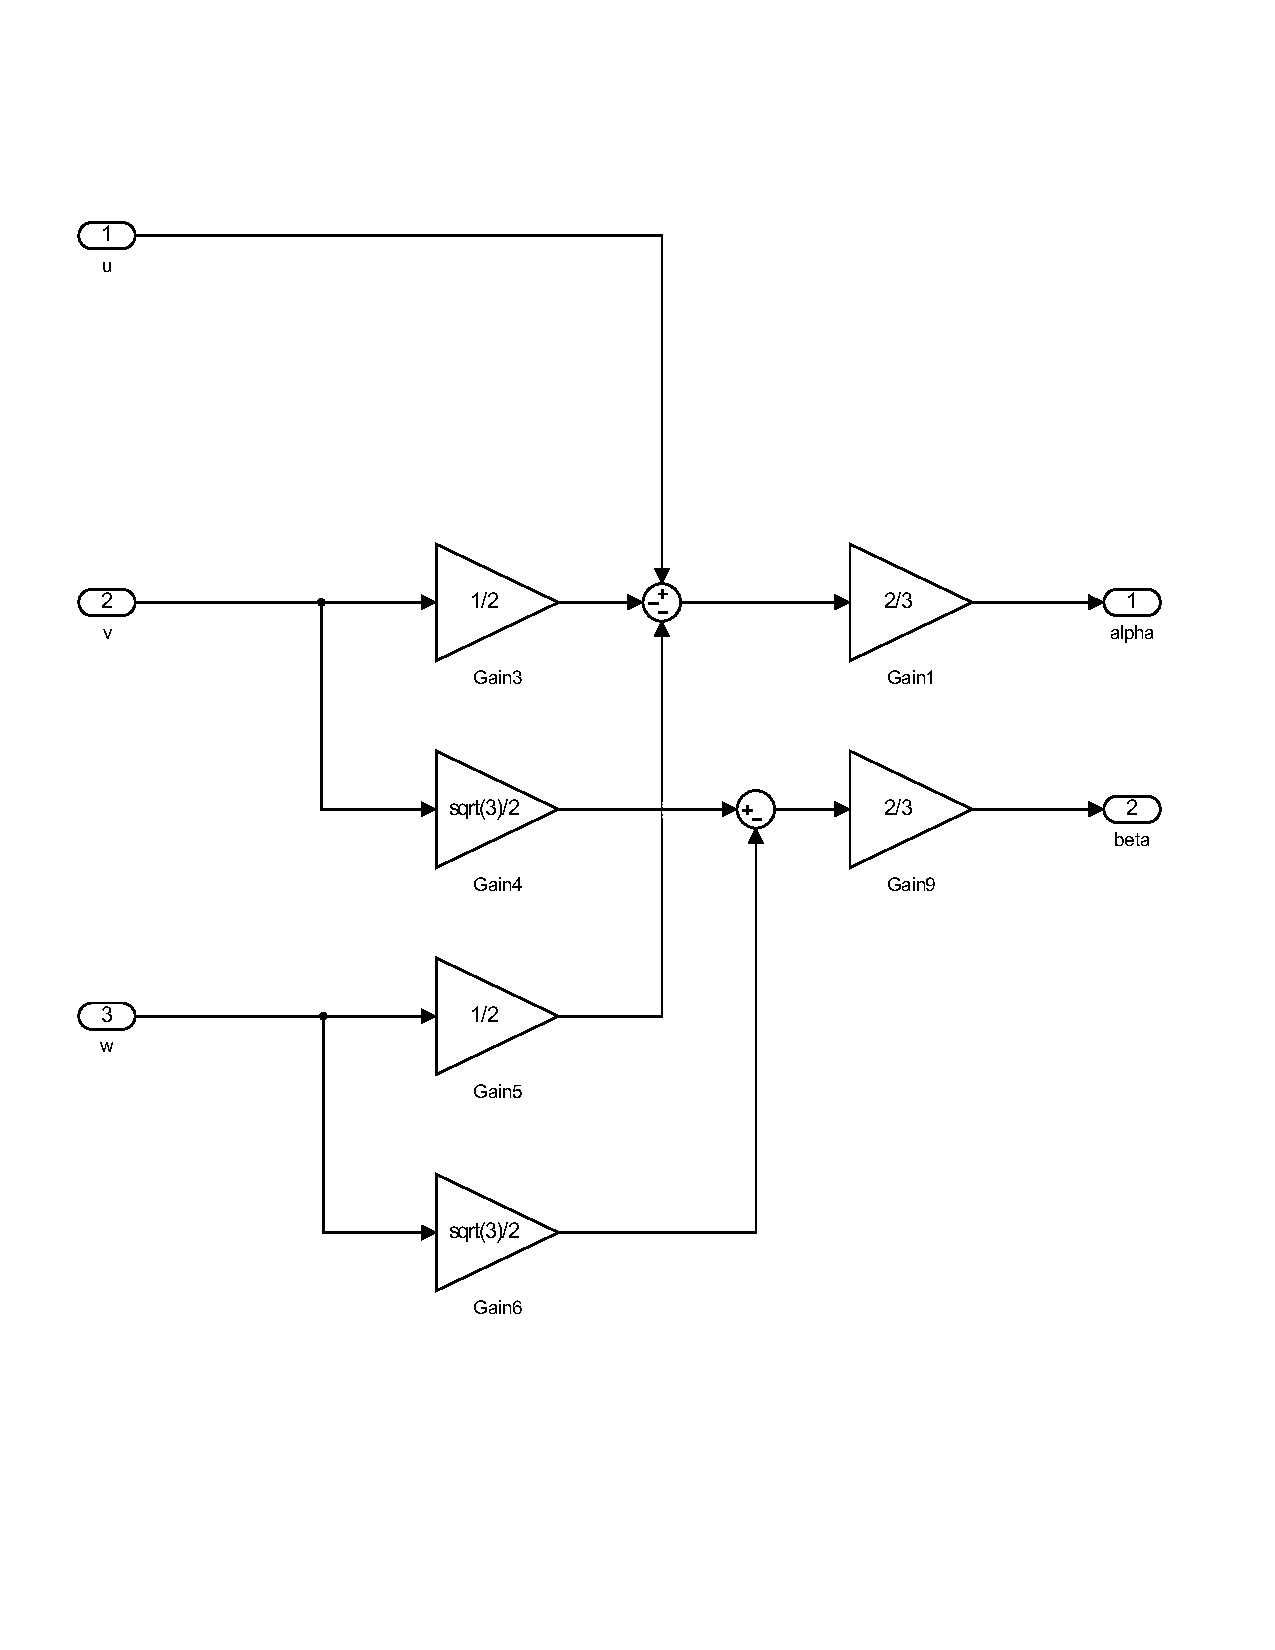
\includegraphics[width=\textwidth]{/simulink/uvw_to_ab.pdf}
	\label{fig:uvw_to_ab}
	\caption{Aufbau der Clarke-Transformation.}
\end{figure}

\begin{figure}[h]
	\centering
	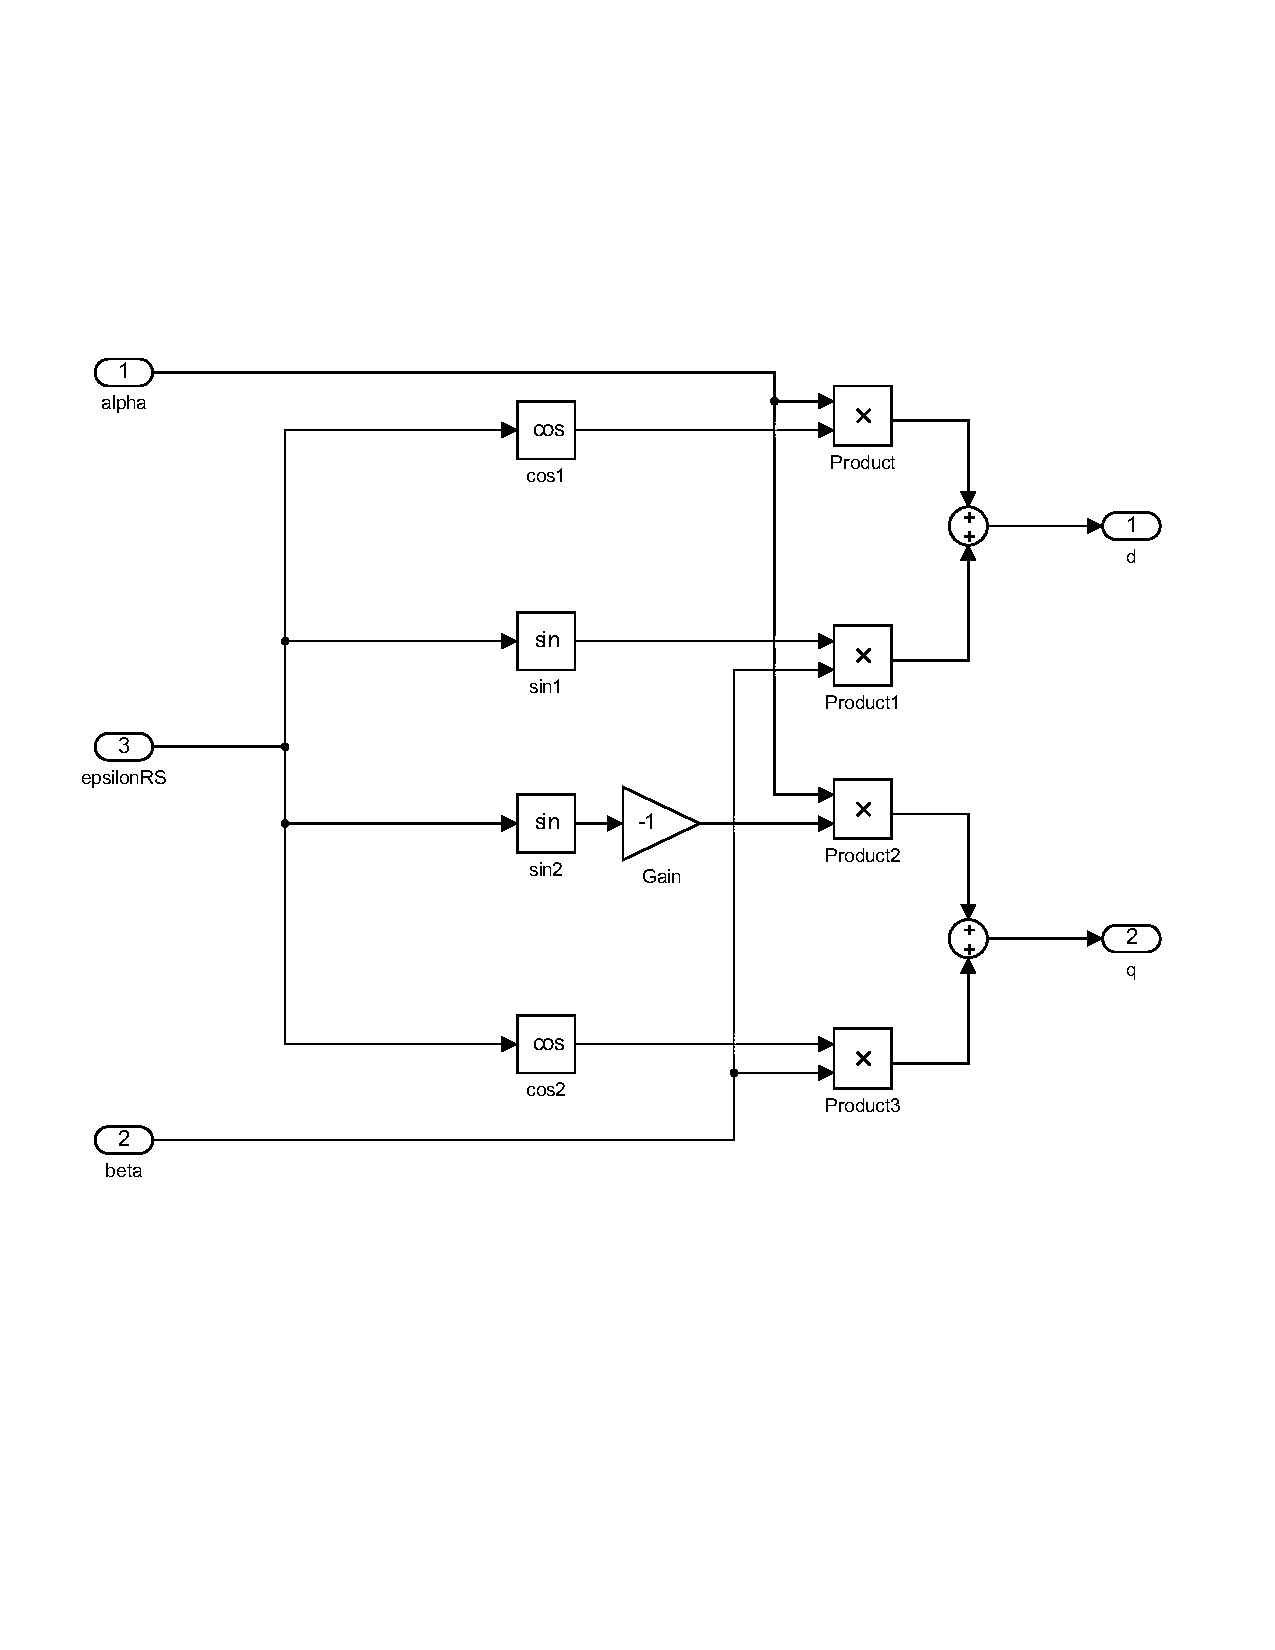
\includegraphics[width=\textwidth]{/simulink/ab_to_dq.pdf}
	\label{fig:uvw_to_ab}
	\caption{Aufbau der Park-Transformation.}
\end{figure}

	
	
\end{appendix}

\end{document}